\documentclass[twoside]{book}

% Packages required by doxygen
\usepackage{fixltx2e}
\usepackage{calc}
\usepackage{doxygen}
\usepackage[export]{adjustbox} % also loads graphicx
\usepackage{graphicx}
\usepackage[utf8]{inputenc}
\usepackage{makeidx}
\usepackage{multicol}
\usepackage{multirow}
\PassOptionsToPackage{warn}{textcomp}
\usepackage{textcomp}
\usepackage[nointegrals]{wasysym}
\usepackage[table]{xcolor}

% Font selection
\usepackage[T1]{fontenc}
\usepackage[scaled=.90]{helvet}
\usepackage{courier}
\usepackage{amssymb}
\usepackage{sectsty}
\renewcommand{\familydefault}{\sfdefault}
\allsectionsfont{%
  \fontseries{bc}\selectfont%
  \color{darkgray}%
}
\renewcommand{\DoxyLabelFont}{%
  \fontseries{bc}\selectfont%
  \color{darkgray}%
}
\newcommand{\+}{\discretionary{\mbox{\scriptsize$\hookleftarrow$}}{}{}}

% Page & text layout
\usepackage{geometry}
\geometry{%
  a4paper,%
  top=2.5cm,%
  bottom=2.5cm,%
  left=2.5cm,%
  right=2.5cm%
}
\tolerance=750
\hfuzz=15pt
\hbadness=750
\setlength{\emergencystretch}{15pt}
\setlength{\parindent}{0cm}
\setlength{\parskip}{3ex plus 2ex minus 2ex}
\makeatletter
\renewcommand{\paragraph}{%
  \@startsection{paragraph}{4}{0ex}{-1.0ex}{1.0ex}{%
    \normalfont\normalsize\bfseries\SS@parafont%
  }%
}
\renewcommand{\subparagraph}{%
  \@startsection{subparagraph}{5}{0ex}{-1.0ex}{1.0ex}{%
    \normalfont\normalsize\bfseries\SS@subparafont%
  }%
}
\makeatother

% Headers & footers
\usepackage{fancyhdr}
\pagestyle{fancyplain}
\fancyhead[LE]{\fancyplain{}{\bfseries\thepage}}
\fancyhead[CE]{\fancyplain{}{}}
\fancyhead[RE]{\fancyplain{}{\bfseries\leftmark}}
\fancyhead[LO]{\fancyplain{}{\bfseries\rightmark}}
\fancyhead[CO]{\fancyplain{}{}}
\fancyhead[RO]{\fancyplain{}{\bfseries\thepage}}
\fancyfoot[LE]{\fancyplain{}{}}
\fancyfoot[CE]{\fancyplain{}{}}
\fancyfoot[RE]{\fancyplain{}{\bfseries\scriptsize Generated by Doxygen }}
\fancyfoot[LO]{\fancyplain{}{\bfseries\scriptsize Generated by Doxygen }}
\fancyfoot[CO]{\fancyplain{}{}}
\fancyfoot[RO]{\fancyplain{}{}}
\renewcommand{\footrulewidth}{0.4pt}
\renewcommand{\chaptermark}[1]{%
  \markboth{#1}{}%
}
\renewcommand{\sectionmark}[1]{%
  \markright{\thesection\ #1}%
}

% Indices & bibliography
\usepackage{natbib}
\usepackage[titles]{tocloft}
\setcounter{tocdepth}{3}
\setcounter{secnumdepth}{5}
\makeindex

% Hyperlinks (required, but should be loaded last)
\usepackage{ifpdf}
\ifpdf
  \usepackage[pdftex,pagebackref=true]{hyperref}
\else
  \usepackage[ps2pdf,pagebackref=true]{hyperref}
\fi
\hypersetup{%
  colorlinks=true,%
  linkcolor=blue,%
  citecolor=blue,%
  unicode%
}

% Custom commands
\newcommand{\clearemptydoublepage}{%
  \newpage{\pagestyle{empty}\cleardoublepage}%
}

\usepackage{caption}
\captionsetup{labelsep=space,justification=centering,font={bf},singlelinecheck=off,skip=4pt,position=top}

%===== C O N T E N T S =====

\begin{document}

% Titlepage & ToC
\hypersetup{pageanchor=false,
             bookmarksnumbered=true,
             pdfencoding=unicode
            }
\pagenumbering{alph}
\begin{titlepage}
\vspace*{7cm}
\begin{center}%
{\Large Keno\+Bet Project }\\
\vspace*{1cm}
{\large Generated by Doxygen 1.8.13}\\
\end{center}
\end{titlepage}
\clearemptydoublepage
\pagenumbering{roman}
\tableofcontents
\clearemptydoublepage
\pagenumbering{arabic}
\hypersetup{pageanchor=true}

%--- Begin generated contents ---
\chapter{Keno\+Bet Index Page}
\label{index}\hypertarget{index}{}\hypertarget{index_intro_sec}{}\section{Introduction}\label{index_intro_sec}
{\bfseries Wellcome to \hyperlink{classKenoBet}{Keno\+Bet} Project} Kenobet is a luck game, you have to pick n numbers in range \mbox{[}0,15) and your pick have ~\newline
 to in the range (1 ,80), place a bet that will be split in n bets rounds, it depends how much hits You get a reward. ~\newline
 \hypertarget{index_install_sec}{}\section{Run}\label{index_install_sec}
\hypertarget{index_step1}{}\subsection{Step 1\+: Make ./keno}\label{index_step1}
g++ -\/\+Wall -\/std=c++11 \hyperlink{main_8cpp}{src/main.\+cpp} \hyperlink{bet_8cpp}{src/bet.\+cpp} -\/I src/ -\/g\hypertarget{index_step2}{}\subsection{Step 2\+: make a bet.\+dat \char`\"{}a bet file\char`\"{}}\label{index_step2}
vim {\bfseries bet.\+dat} ~\newline
 1500 {\bfseries Cash} ~\newline
 3 {\bfseries N} {\bfseries rounds} ~\newline
 20 15 46 {\bfseries You} {\bfseries bets} {\bfseries on} {\bfseries range} {\bfseries }\mbox{[}0 80) ~\newline
 \hypertarget{index_step3}{}\subsection{Step 3\+: Run ./keno}\label{index_step3}
./keno data/bet.\+dat ~\newline
 Dont forgot the place {\bfseries \char`\"{}\+Bet F\+I\+L\+E\char`\"{}}  \hypertarget{index_step4}{}\subsection{Step 4\+: Game Running}\label{index_step4}
press {\bfseries Enter} ~\newline
 to pass rounds~\newline
 in the end you can continue playe ~\newline
 press {\bfseries 1} set a new {\bfseries bet} {\bfseries F\+Ile} ~\newline
\hypertarget{index_step5}{}\subsection{E\+R\+R\+O\+S\+: valgrid issues}\label{index_step5}
==4332== Invalid read of size 1 ~\newline
==4332== at 0x4\+C32\+D32\+: \+\_\+\+\_\+strlen\+\_\+sse2 (in /usr/lib/valgrind/vgpreload\+\_\+memcheck-\/amd64-\/linux.so)~\newline
==4332== by 0x4\+F61\+C93\+: std\+::\+\_\+\+\_\+cxx11\+::basic\+\_\+string$<$char, std\+::char\+\_\+traits$<$char$>$, std\+::allocator$<$char$>$ $>$\+::operator=(char const$\ast$) (in /usr/lib/x86\+\_\+64-\/linux-\/gnu/libstdc++.so.\+6.\+0.\+25) ~\newline
==4332== by 0x1099\+F3\+: main (\hyperlink{main_8cpp}{main.\+cpp}\+:14)~\newline
==4332== Address 0x0 is not stack\textquotesingle{}d, malloc\textquotesingle{}d or (recently) free\textquotesingle{}d ~\newline
Error convert in=argv\mbox{[}i\mbox{]}\hypertarget{index_step6}{}\subsection{E\+R\+R\+O\+S\+: Bet\+File Issues}\label{index_step6}
The B\+E\+T\+F\+I\+LE must have one white-\/space bet between spots. 
\chapter{Class Index}
\section{Class List}
Here are the classes, structs, unions and interfaces with brief descriptions\+:\begin{DoxyCompactList}
\item\contentsline{section}{\hyperlink{classKenoBet}{Keno\+Bet} }{\pageref{classKenoBet}}{}
\end{DoxyCompactList}

\chapter{File Index}
\section{File List}
Here is a list of all files with brief descriptions\+:\begin{DoxyCompactList}
\item\contentsline{section}{/home/bergony/lp\+\_\+projeto\+\_\+keno/include/\hyperlink{bet_8h}{bet.\+h} }{\pageref{bet_8h}}{}
\item\contentsline{section}{/home/bergony/lp\+\_\+projeto\+\_\+keno/src/\hyperlink{bet_8cpp}{bet.\+cpp} }{\pageref{bet_8cpp}}{}
\item\contentsline{section}{/home/bergony/lp\+\_\+projeto\+\_\+keno/src/\hyperlink{main_8cpp}{main.\+cpp} }{\pageref{main_8cpp}}{}
\end{DoxyCompactList}

\chapter{Class Documentation}
\hypertarget{classKenoBet}{}\section{Keno\+Bet Class Reference}
\label{classKenoBet}\index{Keno\+Bet@{Keno\+Bet}}


{\ttfamily \#include $<$bet.\+h$>$}

\subsection*{Public Member Functions}
\begin{DoxyCompactItemize}
\item 
\hyperlink{classKenoBet_a225e9428e2bc69acfd4fef3effdd4ccc}{Keno\+Bet} (float i=0, float t=0, float s=0, float ts=0, int n=0)
\begin{DoxyCompactList}\small\item\em ! Constructor Keno bet . \end{DoxyCompactList}\item 
\hyperlink{classKenoBet_aed0e6361718c05a48c1be8653ffcf2d4}{$\sim$\+Keno\+Bet} (void)
\begin{DoxyCompactList}\small\item\em ! Destructor Keno Bet \end{DoxyCompactList}\item 
\hyperlink{classKenoBet_aaabc53c7d5505c3aae1de7b685f72f05}{Keno\+Bet} (const \hyperlink{classKenoBet}{Keno\+Bet} \&clone)
\begin{DoxyCompactList}\small\item\em ! Copy Keno Bet \end{DoxyCompactList}\item 
float \hyperlink{classKenoBet_aace00d82c42c9870a4f3b95c7ec79f24}{get\+\_\+\+IC} (void) const
\begin{DoxyCompactList}\small\item\em Get Inital Cash. \end{DoxyCompactList}\item 
float \hyperlink{classKenoBet_ade294f6dcb57c7a55be5ce2303664b0a}{get\+\_\+\+TC} (void) const
\begin{DoxyCompactList}\small\item\em Get Total Cash. \end{DoxyCompactList}\item 
float \hyperlink{classKenoBet_a0c2ee88fc2f8e7afc5b0399fe74c022b}{get\+\_\+\+SC} (void) const
\begin{DoxyCompactList}\small\item\em Get Spend Cash per Round. \end{DoxyCompactList}\item 
float \hyperlink{classKenoBet_a15782d60d2e9b76f359963865a714a04}{get\+\_\+\+T\+SC} (void) const
\begin{DoxyCompactList}\small\item\em Get Total Inital Cash. \end{DoxyCompactList}\item 
int \hyperlink{classKenoBet_a79f26e472d9a60894e25094a37d06eb6}{get\+\_\+spot\+\_\+r} (void)
\begin{DoxyCompactList}\small\item\em Get Valor of Hits Right. \end{DoxyCompactList}\item 
int $\ast$ \hyperlink{classKenoBet_a386ab5f7108fd2df3518f37bfca2b2ef}{get\+\_\+m\+\_\+spots} (void)
\begin{DoxyCompactList}\small\item\em Get Pointer of begin vector(spots) \end{DoxyCompactList}\item 
int $\ast$ \hyperlink{classKenoBet_a8106aa1f149ba3043a8219453e1af3a1}{get\+\_\+m\+\_\+spots\+\_\+rdn} (void)
\begin{DoxyCompactList}\small\item\em Get Pointer of begin vector(spots\+\_\+rdn) \end{DoxyCompactList}\item 
int $\ast$ \hyperlink{classKenoBet_a1a124437ed672df3e4e7d195d9716540}{get\+\_\+m\+\_\+spots\+\_\+r} (void)
\begin{DoxyCompactList}\small\item\em Get Pointer of begin vector(spots\+\_\+r) \end{DoxyCompactList}\item 
void \hyperlink{classKenoBet_a7b74641d226e6b2ea45bc60889f32781}{set\+\_\+\+IC} (const float \&n\+\_\+\+IC)
\begin{DoxyCompactList}\small\item\em !\+Set Inital Cash. \end{DoxyCompactList}\item 
void \hyperlink{classKenoBet_aa9be1ef95a09fcc293e7c73e763ff176}{set\+\_\+\+TC} (const float \&n\+\_\+\+TC)
\begin{DoxyCompactList}\small\item\em !\+Set Total Cash \end{DoxyCompactList}\item 
void \hyperlink{classKenoBet_a4865fd866acc1500bde749d8d15ddf16}{set\+\_\+\+SC} (const float \&n\+\_\+\+SC)
\begin{DoxyCompactList}\small\item\em !\+Set Spend Cash per round. \end{DoxyCompactList}\item 
void \hyperlink{classKenoBet_abd6b6b0b0ed9c3d030a71673dc89f39a}{set\+\_\+\+T\+SC} (const float \&n\+\_\+\+T\+SC)
\begin{DoxyCompactList}\small\item\em !set Total Spend Cash. \end{DoxyCompactList}\item 
void \hyperlink{classKenoBet_a63780c5d19157760a2760407cd68149f}{set\+\_\+\+NR} (const int \&n\+\_\+\+NR)
\begin{DoxyCompactList}\small\item\em !\+Set Numbers Rounds. \end{DoxyCompactList}\item 
void \hyperlink{classKenoBet_acdeff501accf00661e0151901bc888c0}{set\+\_\+spot\+\_\+h} (int n\+\_\+spot\+\_\+r)
\begin{DoxyCompactList}\small\item\em !\+Set valor of hits right. \end{DoxyCompactList}\item 
bool \hyperlink{classKenoBet_aba848a50d30a0155459eb9f5cbb91966}{add\+\_\+number} (int spot\+\_\+)
\begin{DoxyCompactList}\small\item\em Adds a number to the spots only if the number is not already there. \end{DoxyCompactList}\item 
bool \hyperlink{classKenoBet_a2b21e387cde33818230d9895845b2d9a}{set\+\_\+wage} (float wage\+\_\+)
\begin{DoxyCompactList}\small\item\em Sets the amount of money the player is betting. \end{DoxyCompactList}\item 
void \hyperlink{classKenoBet_acc2afd4d502e44fdfbb122f3389bc633}{reset} (void)
\begin{DoxyCompactList}\small\item\em ! Resets a bet to an empty state. \end{DoxyCompactList}\item 
float \hyperlink{classKenoBet_a65f0348e49dd8a2e2dddfcc9a1f05a65}{get\+\_\+wage} (void) const
\begin{DoxyCompactList}\small\item\em Retrieves the player ’s wage on this bet . \end{DoxyCompactList}\item 
size\+\_\+t \hyperlink{classKenoBet_aa6f65b35514270c2707e60b9dea23ae9}{size} (void) const
\begin{DoxyCompactList}\small\item\em Returns to the current number of spots in the player ’s bet. \end{DoxyCompactList}\item 
std\+::vector$<$ int $>$ \hyperlink{classKenoBet_a382454c66974466900d168c398699483}{get\+\_\+spots} (void) const
\begin{DoxyCompactList}\small\item\em Return a vector $<$ spot\+\_\+type $>$ with the spots the player has picked so far. \end{DoxyCompactList}\item 
std\+::vector$<$ int $>$ \hyperlink{classKenoBet_a612b57c35203a41682269cdfbb31c2b1}{get\+\_\+hits} (const std\+::vector$<$ int $>$ \&hits\+\_\+)
\begin{DoxyCompactList}\small\item\em Determine how many spots match the hits passed as argument . \end{DoxyCompactList}\item 
void \hyperlink{classKenoBet_aa2093fa2b053cf74e95d1e6b54d748f3}{hits\+\_\+rdn} (void)
\begin{DoxyCompactList}\small\item\em Randon Hits. \end{DoxyCompactList}\item 
unsigned int \hyperlink{classKenoBet_a5a544a0c1ba5872076e7bfdf8f935368}{operator\mbox{[}$\,$\mbox{]}} (int n)
\begin{DoxyCompactList}\small\item\em operator\mbox{[}\mbox{]} \end{DoxyCompactList}\end{DoxyCompactItemize}


\subsection{Constructor \& Destructor Documentation}
\mbox{\Hypertarget{classKenoBet_a225e9428e2bc69acfd4fef3effdd4ccc}\label{classKenoBet_a225e9428e2bc69acfd4fef3effdd4ccc}} 
\index{Keno\+Bet@{Keno\+Bet}!Keno\+Bet@{Keno\+Bet}}
\index{Keno\+Bet@{Keno\+Bet}!Keno\+Bet@{Keno\+Bet}}
\subsubsection{\texorpdfstring{Keno\+Bet()}{KenoBet()}\hspace{0.1cm}{\footnotesize\ttfamily [1/2]}}
{\footnotesize\ttfamily Keno\+Bet\+::\+Keno\+Bet (\begin{DoxyParamCaption}\item[{float}]{i = {\ttfamily 0},  }\item[{float}]{t = {\ttfamily 0},  }\item[{float}]{s = {\ttfamily 0},  }\item[{float}]{ts = {\ttfamily 0},  }\item[{int}]{n = {\ttfamily 0} }\end{DoxyParamCaption})\hspace{0.3cm}{\ttfamily [inline]}}



! Constructor Keno bet . 


\begin{DoxyCode}
15             :    m\_IC\{ i \}, m\_TC\{ t \}, m\_SC\{ s \}, m\_TSC\{ ts \}, m\_NR\{ n \}
16         \{
17             \textcolor{comment}{/* empty */}
18         \}
\end{DoxyCode}
\mbox{\Hypertarget{classKenoBet_aed0e6361718c05a48c1be8653ffcf2d4}\label{classKenoBet_aed0e6361718c05a48c1be8653ffcf2d4}} 
\index{Keno\+Bet@{Keno\+Bet}!````~Keno\+Bet@{$\sim$\+Keno\+Bet}}
\index{````~Keno\+Bet@{$\sim$\+Keno\+Bet}!Keno\+Bet@{Keno\+Bet}}
\subsubsection{\texorpdfstring{$\sim$\+Keno\+Bet()}{~KenoBet()}}
{\footnotesize\ttfamily Keno\+Bet\+::$\sim$\+Keno\+Bet (\begin{DoxyParamCaption}\item[{void}]{ }\end{DoxyParamCaption})\hspace{0.3cm}{\ttfamily [inline]}}



! Destructor Keno Bet 


\begin{DoxyCode}
21         \{
22             \textcolor{comment}{/* empty */}
23         \}
\end{DoxyCode}
\mbox{\Hypertarget{classKenoBet_aaabc53c7d5505c3aae1de7b685f72f05}\label{classKenoBet_aaabc53c7d5505c3aae1de7b685f72f05}} 
\index{Keno\+Bet@{Keno\+Bet}!Keno\+Bet@{Keno\+Bet}}
\index{Keno\+Bet@{Keno\+Bet}!Keno\+Bet@{Keno\+Bet}}
\subsubsection{\texorpdfstring{Keno\+Bet()}{KenoBet()}\hspace{0.1cm}{\footnotesize\ttfamily [2/2]}}
{\footnotesize\ttfamily Keno\+Bet\+::\+Keno\+Bet (\begin{DoxyParamCaption}\item[{const \hyperlink{classKenoBet}{Keno\+Bet} \&}]{clone }\end{DoxyParamCaption})\hspace{0.3cm}{\ttfamily [inline]}}



! Copy Keno Bet 


\begin{DoxyCode}
26         \{
27             m\_IC = clone.m\_IC;
28             m\_TC = clone.m\_TC;
29             m\_SC = clone.m\_SC;
30             m\_NR = clone.m\_NR;
31             m\_spots = clone.m\_spots;
32         \}
\end{DoxyCode}
Here is the call graph for this function\+:
\nopagebreak
\begin{figure}[H]
\begin{center}
\leavevmode
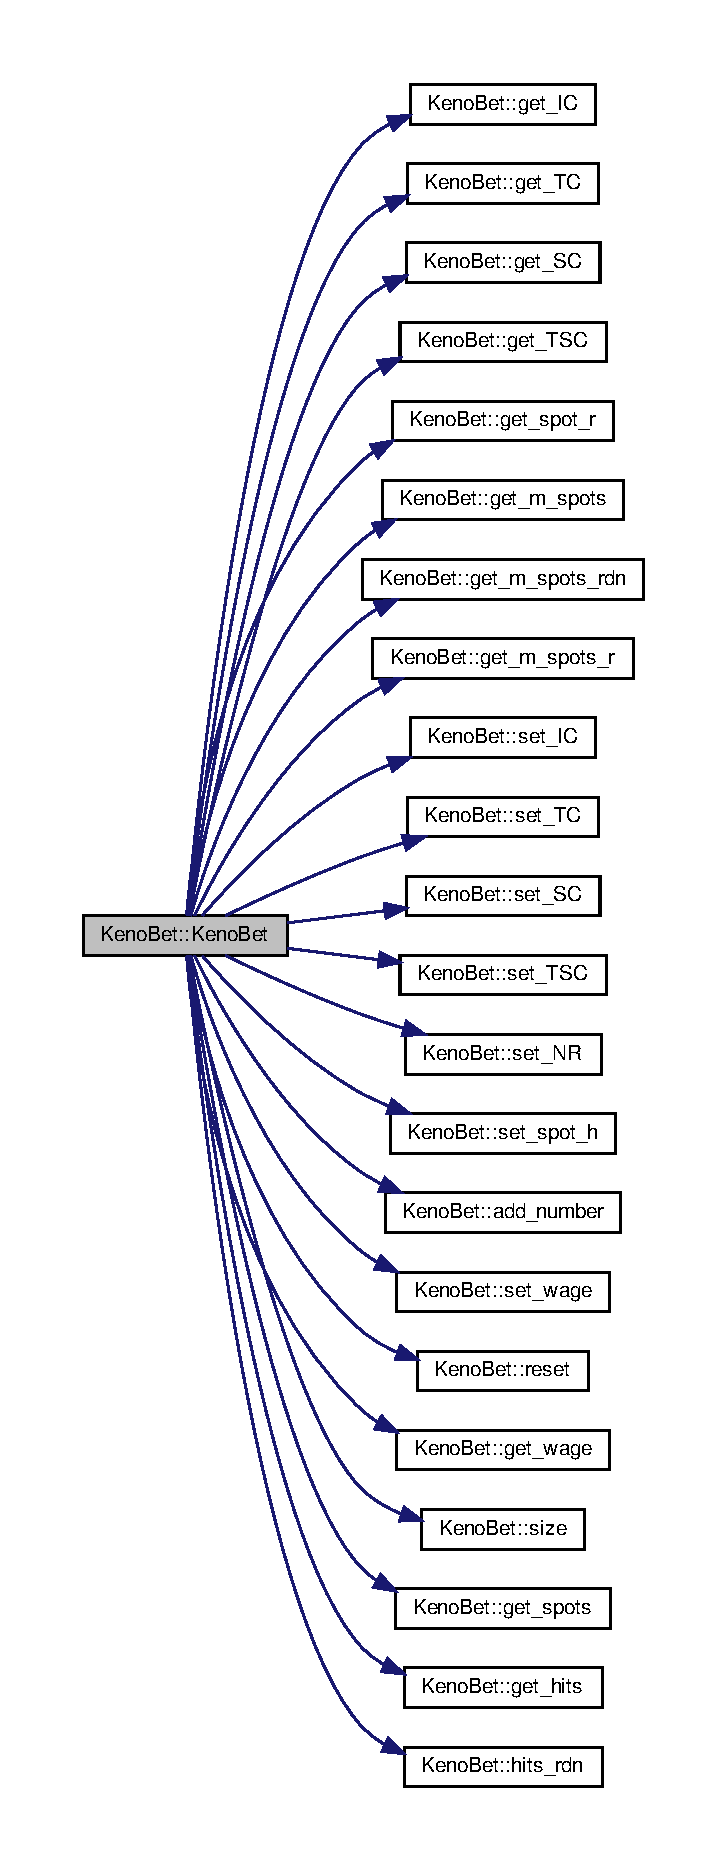
\includegraphics[height=550pt]{classKenoBet_aaabc53c7d5505c3aae1de7b685f72f05_cgraph}
\end{center}
\end{figure}


\subsection{Member Function Documentation}
\mbox{\Hypertarget{classKenoBet_aba848a50d30a0155459eb9f5cbb91966}\label{classKenoBet_aba848a50d30a0155459eb9f5cbb91966}} 
\index{Keno\+Bet@{Keno\+Bet}!add\+\_\+number@{add\+\_\+number}}
\index{add\+\_\+number@{add\+\_\+number}!Keno\+Bet@{Keno\+Bet}}
\subsubsection{\texorpdfstring{add\+\_\+number()}{add\_number()}}
{\footnotesize\ttfamily bool Keno\+Bet\+::add\+\_\+number (\begin{DoxyParamCaption}\item[{int}]{spot\+\_\+ }\end{DoxyParamCaption})}



Adds a number to the spots only if the number is not already there. 


\begin{DoxyParams}{Parameters}
{\em spot\+\_\+} & The number we wish to include in the bet . \\
\hline
\end{DoxyParams}
\begin{DoxyReturn}{Returns}
True if number chosen is successfully inserted ; False otherwise. 
\end{DoxyReturn}

\begin{DoxyCode}
160 \{
161     \textcolor{keywordtype}{int} index\{0\};
162     \textcolor{keywordflow}{while}( m\_spots.begin() + index != m\_spots.end() )
163     \{
164         \textcolor{keywordflow}{if}( spot\_ == *(m\_spots.begin()+index) )
165         \{
166             \textcolor{keywordflow}{return} \textcolor{keyword}{false};
167         \}
168         index++;
169     \}
170     m\_spots.push\_back(spot\_);
171     \textcolor{keywordflow}{return} \textcolor{keyword}{true};
172 \}
\end{DoxyCode}
Here is the caller graph for this function\+:
\nopagebreak
\begin{figure}[H]
\begin{center}
\leavevmode
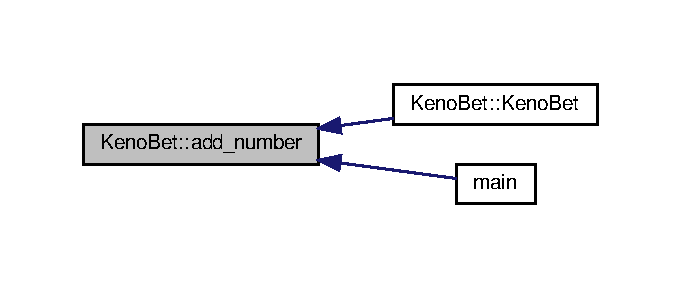
\includegraphics[width=327pt]{classKenoBet_aba848a50d30a0155459eb9f5cbb91966_icgraph}
\end{center}
\end{figure}
\mbox{\Hypertarget{classKenoBet_a612b57c35203a41682269cdfbb31c2b1}\label{classKenoBet_a612b57c35203a41682269cdfbb31c2b1}} 
\index{Keno\+Bet@{Keno\+Bet}!get\+\_\+hits@{get\+\_\+hits}}
\index{get\+\_\+hits@{get\+\_\+hits}!Keno\+Bet@{Keno\+Bet}}
\subsubsection{\texorpdfstring{get\+\_\+hits()}{get\_hits()}}
{\footnotesize\ttfamily std\+::vector$<$ int $>$ Keno\+Bet\+::get\+\_\+hits (\begin{DoxyParamCaption}\item[{const std\+::vector$<$ int $>$ \&}]{hits\+\_\+ }\end{DoxyParamCaption})}



Determine how many spots match the hits passed as argument . 


\begin{DoxyParams}{Parameters}
{\em hits\+\_\+} & List of hits randomly chosen by the computer . \\
\hline
\end{DoxyParams}
\begin{DoxyReturn}{Returns}
An vector with the list of hits . 
\end{DoxyReturn}

\begin{DoxyCode}
197 \{
198     srand(time(NULL));
199     \textcolor{keywordtype}{int} index\{0\};
200     \textcolor{keywordtype}{bool} repeat\{\textcolor{keyword}{false}\};
201 
202     \textcolor{keyword}{auto} save\_rand = rand() % 80+1;
203     \textcolor{keywordflow}{for}(\textcolor{keywordtype}{int} i\{0\};i < 20; )
204     \{
205         save\_rand = rand() % 80+1;
206         index = 0;
207         repeat = \textcolor{keyword}{false};
208 
209         \textcolor{keywordflow}{while}(m\_spots\_rdn.begin()+index != m\_spots\_rdn.end() )
210         \{
211             \textcolor{keywordflow}{if}(save\_rand == *(m\_spots\_rdn.begin()+index))
212                 repeat = \textcolor{keyword}{true};
213             index++;
214         \}
215         \textcolor{keywordflow}{if}(repeat == \textcolor{keyword}{false})
216         \{
217             m\_spots\_rdn.push\_back( save\_rand );
218             i++;
219         \}
220     \}
221     \textcolor{keywordflow}{for}(\textcolor{keywordtype}{int} i\{0\};i < m\_NR; i++)
222     \{
223         \textcolor{keywordflow}{for}(\textcolor{keywordtype}{int} j\{0\}; j < 20; j++)
224         \{
225             \textcolor{keywordflow}{if}(*(m\_spots.begin()+i) == *(m\_spots\_rdn.begin()+j))
226                 m\_spots\_r.push\_back( *(m\_spots.begin()+i) );
227         \}
228     \}
229     \textcolor{keywordflow}{return} m\_spots\_r;
230 \}
\end{DoxyCode}
Here is the caller graph for this function\+:
\nopagebreak
\begin{figure}[H]
\begin{center}
\leavevmode
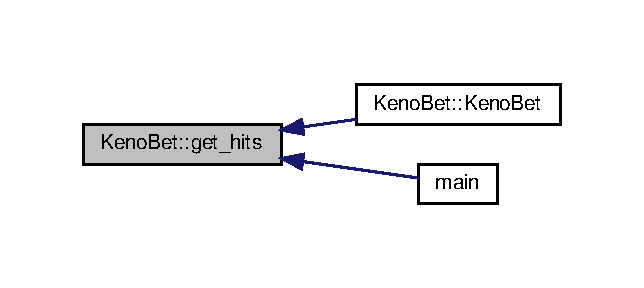
\includegraphics[width=309pt]{classKenoBet_a612b57c35203a41682269cdfbb31c2b1_icgraph}
\end{center}
\end{figure}
\mbox{\Hypertarget{classKenoBet_aace00d82c42c9870a4f3b95c7ec79f24}\label{classKenoBet_aace00d82c42c9870a4f3b95c7ec79f24}} 
\index{Keno\+Bet@{Keno\+Bet}!get\+\_\+\+IC@{get\+\_\+\+IC}}
\index{get\+\_\+\+IC@{get\+\_\+\+IC}!Keno\+Bet@{Keno\+Bet}}
\subsubsection{\texorpdfstring{get\+\_\+\+I\+C()}{get\_IC()}}
{\footnotesize\ttfamily float Keno\+Bet\+::get\+\_\+\+IC (\begin{DoxyParamCaption}\item[{void}]{ }\end{DoxyParamCaption}) const}



Get Inital Cash. 

\begin{DoxyReturn}{Returns}
Valor of Inital Cash. 
\end{DoxyReturn}

\begin{DoxyCode}
111 \{
112     \textcolor{keywordflow}{return} m\_IC;
113 \}
\end{DoxyCode}
Here is the caller graph for this function\+:
\nopagebreak
\begin{figure}[H]
\begin{center}
\leavevmode
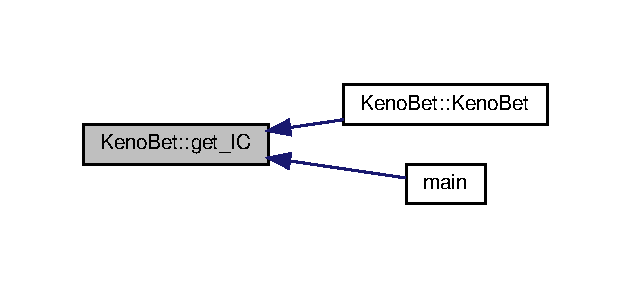
\includegraphics[width=303pt]{classKenoBet_aace00d82c42c9870a4f3b95c7ec79f24_icgraph}
\end{center}
\end{figure}
\mbox{\Hypertarget{classKenoBet_a386ab5f7108fd2df3518f37bfca2b2ef}\label{classKenoBet_a386ab5f7108fd2df3518f37bfca2b2ef}} 
\index{Keno\+Bet@{Keno\+Bet}!get\+\_\+m\+\_\+spots@{get\+\_\+m\+\_\+spots}}
\index{get\+\_\+m\+\_\+spots@{get\+\_\+m\+\_\+spots}!Keno\+Bet@{Keno\+Bet}}
\subsubsection{\texorpdfstring{get\+\_\+m\+\_\+spots()}{get\_m\_spots()}}
{\footnotesize\ttfamily int $\ast$ Keno\+Bet\+::get\+\_\+m\+\_\+spots (\begin{DoxyParamCaption}\item[{void}]{ }\end{DoxyParamCaption})}



Get Pointer of begin vector(spots) 

\begin{DoxyReturn}{Returns}
Pointer to begin of vector. 
\end{DoxyReturn}

\begin{DoxyCode}
188 \{
189     \textcolor{keywordflow}{return} &(*m\_spots.begin());
190 \}
\end{DoxyCode}
Here is the caller graph for this function\+:
\nopagebreak
\begin{figure}[H]
\begin{center}
\leavevmode
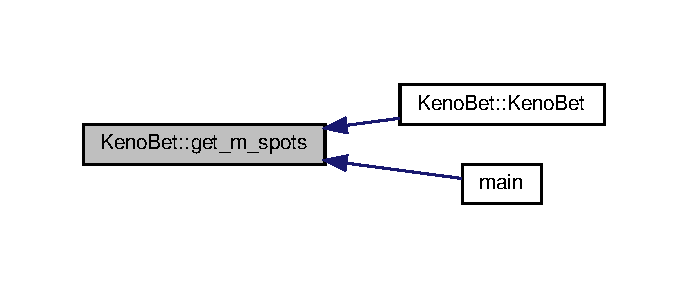
\includegraphics[width=330pt]{classKenoBet_a386ab5f7108fd2df3518f37bfca2b2ef_icgraph}
\end{center}
\end{figure}
\mbox{\Hypertarget{classKenoBet_a1a124437ed672df3e4e7d195d9716540}\label{classKenoBet_a1a124437ed672df3e4e7d195d9716540}} 
\index{Keno\+Bet@{Keno\+Bet}!get\+\_\+m\+\_\+spots\+\_\+r@{get\+\_\+m\+\_\+spots\+\_\+r}}
\index{get\+\_\+m\+\_\+spots\+\_\+r@{get\+\_\+m\+\_\+spots\+\_\+r}!Keno\+Bet@{Keno\+Bet}}
\subsubsection{\texorpdfstring{get\+\_\+m\+\_\+spots\+\_\+r()}{get\_m\_spots\_r()}}
{\footnotesize\ttfamily int $\ast$ Keno\+Bet\+::get\+\_\+m\+\_\+spots\+\_\+r (\begin{DoxyParamCaption}\item[{void}]{ }\end{DoxyParamCaption})}



Get Pointer of begin vector(spots\+\_\+r) 

\begin{DoxyReturn}{Returns}
Pointer to begin of vector. 
\end{DoxyReturn}

\begin{DoxyCode}
192 \{
193     \textcolor{keywordflow}{return} &(*m\_spots\_r.begin());
194 \}
\end{DoxyCode}
Here is the caller graph for this function\+:
\nopagebreak
\begin{figure}[H]
\begin{center}
\leavevmode
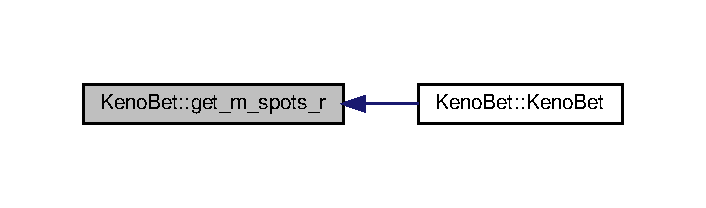
\includegraphics[width=339pt]{classKenoBet_a1a124437ed672df3e4e7d195d9716540_icgraph}
\end{center}
\end{figure}
\mbox{\Hypertarget{classKenoBet_a8106aa1f149ba3043a8219453e1af3a1}\label{classKenoBet_a8106aa1f149ba3043a8219453e1af3a1}} 
\index{Keno\+Bet@{Keno\+Bet}!get\+\_\+m\+\_\+spots\+\_\+rdn@{get\+\_\+m\+\_\+spots\+\_\+rdn}}
\index{get\+\_\+m\+\_\+spots\+\_\+rdn@{get\+\_\+m\+\_\+spots\+\_\+rdn}!Keno\+Bet@{Keno\+Bet}}
\subsubsection{\texorpdfstring{get\+\_\+m\+\_\+spots\+\_\+rdn()}{get\_m\_spots\_rdn()}}
{\footnotesize\ttfamily int $\ast$ Keno\+Bet\+::get\+\_\+m\+\_\+spots\+\_\+rdn (\begin{DoxyParamCaption}\item[{void}]{ }\end{DoxyParamCaption})}



Get Pointer of begin vector(spots\+\_\+rdn) 

\begin{DoxyReturn}{Returns}
Pointer to begin of vector. 
\end{DoxyReturn}

\begin{DoxyCode}
184 \{
185     \textcolor{keywordflow}{return} &(*m\_spots\_rdn.begin());
186 \}
\end{DoxyCode}
Here is the caller graph for this function\+:
\nopagebreak
\begin{figure}[H]
\begin{center}
\leavevmode
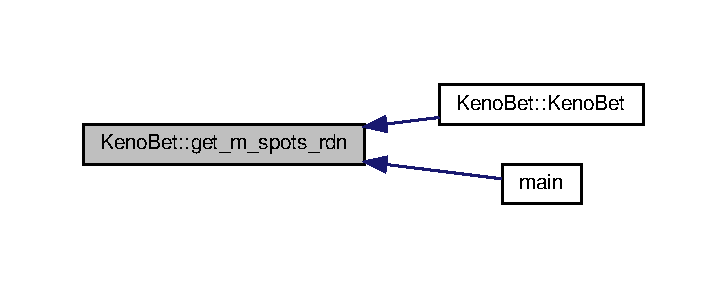
\includegraphics[width=349pt]{classKenoBet_a8106aa1f149ba3043a8219453e1af3a1_icgraph}
\end{center}
\end{figure}
\mbox{\Hypertarget{classKenoBet_a0c2ee88fc2f8e7afc5b0399fe74c022b}\label{classKenoBet_a0c2ee88fc2f8e7afc5b0399fe74c022b}} 
\index{Keno\+Bet@{Keno\+Bet}!get\+\_\+\+SC@{get\+\_\+\+SC}}
\index{get\+\_\+\+SC@{get\+\_\+\+SC}!Keno\+Bet@{Keno\+Bet}}
\subsubsection{\texorpdfstring{get\+\_\+\+S\+C()}{get\_SC()}}
{\footnotesize\ttfamily float Keno\+Bet\+::get\+\_\+\+SC (\begin{DoxyParamCaption}\item[{void}]{ }\end{DoxyParamCaption}) const}



Get Spend Cash per Round. 

\begin{DoxyReturn}{Returns}
Valor of Spend Cash per round. 
\end{DoxyReturn}

\begin{DoxyCode}
119 \{
120     \textcolor{keywordflow}{return} m\_SC;
121 \}
\end{DoxyCode}
Here is the caller graph for this function\+:
\nopagebreak
\begin{figure}[H]
\begin{center}
\leavevmode
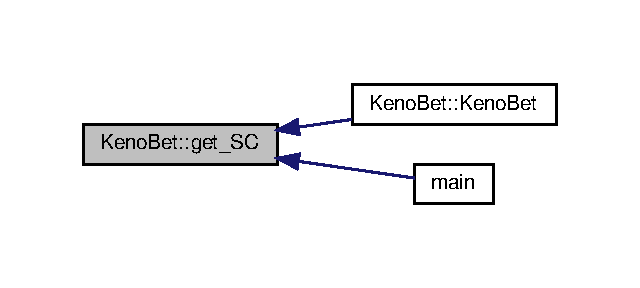
\includegraphics[width=307pt]{classKenoBet_a0c2ee88fc2f8e7afc5b0399fe74c022b_icgraph}
\end{center}
\end{figure}
\mbox{\Hypertarget{classKenoBet_a79f26e472d9a60894e25094a37d06eb6}\label{classKenoBet_a79f26e472d9a60894e25094a37d06eb6}} 
\index{Keno\+Bet@{Keno\+Bet}!get\+\_\+spot\+\_\+r@{get\+\_\+spot\+\_\+r}}
\index{get\+\_\+spot\+\_\+r@{get\+\_\+spot\+\_\+r}!Keno\+Bet@{Keno\+Bet}}
\subsubsection{\texorpdfstring{get\+\_\+spot\+\_\+r()}{get\_spot\_r()}}
{\footnotesize\ttfamily int Keno\+Bet\+::get\+\_\+spot\+\_\+r (\begin{DoxyParamCaption}\item[{void}]{ }\end{DoxyParamCaption})}



Get Valor of Hits Right. 

\begin{DoxyReturn}{Returns}
Valor of Hits Right. 
\end{DoxyReturn}

\begin{DoxyCode}
236 \{
237     \textcolor{keywordtype}{int} index\{0\};
238     \textcolor{keywordflow}{while}(m\_spots\_r.begin()+index != m\_spots\_r.end() )
239     \{
240         index++;
241     \}
242     \textcolor{keywordflow}{return} index;
243 \}
\end{DoxyCode}
Here is the caller graph for this function\+:
\nopagebreak
\begin{figure}[H]
\begin{center}
\leavevmode
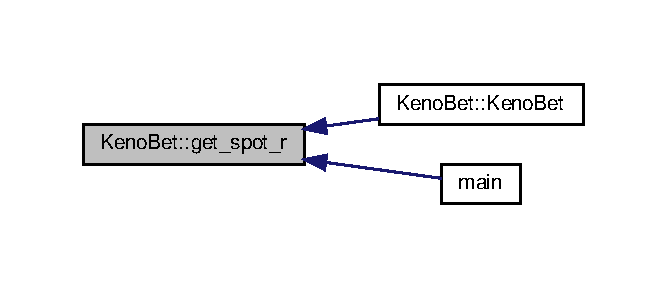
\includegraphics[width=320pt]{classKenoBet_a79f26e472d9a60894e25094a37d06eb6_icgraph}
\end{center}
\end{figure}
\mbox{\Hypertarget{classKenoBet_a382454c66974466900d168c398699483}\label{classKenoBet_a382454c66974466900d168c398699483}} 
\index{Keno\+Bet@{Keno\+Bet}!get\+\_\+spots@{get\+\_\+spots}}
\index{get\+\_\+spots@{get\+\_\+spots}!Keno\+Bet@{Keno\+Bet}}
\subsubsection{\texorpdfstring{get\+\_\+spots()}{get\_spots()}}
{\footnotesize\ttfamily std\+::vector$<$ int $>$ Keno\+Bet\+::get\+\_\+spots (\begin{DoxyParamCaption}\item[{void}]{ }\end{DoxyParamCaption}) const}



Return a vector $<$ spot\+\_\+type $>$ with the spots the player has picked so far. 

\begin{DoxyReturn}{Returns}
The vector $<$ spot\+\_\+type $>$ with the player ’s spots picked so far. 
\end{DoxyReturn}

\begin{DoxyCode}
232 \{
233     \textcolor{keywordflow}{return} m\_spots;
234 \}
\end{DoxyCode}
Here is the caller graph for this function\+:
\nopagebreak
\begin{figure}[H]
\begin{center}
\leavevmode
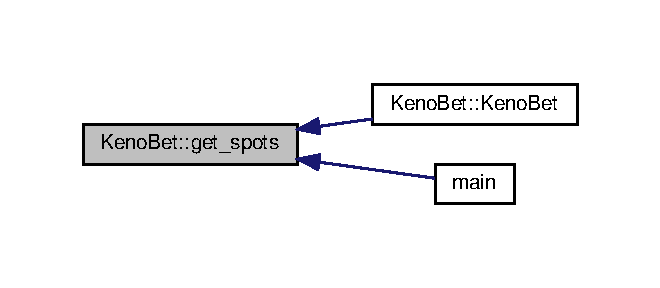
\includegraphics[width=317pt]{classKenoBet_a382454c66974466900d168c398699483_icgraph}
\end{center}
\end{figure}
\mbox{\Hypertarget{classKenoBet_ade294f6dcb57c7a55be5ce2303664b0a}\label{classKenoBet_ade294f6dcb57c7a55be5ce2303664b0a}} 
\index{Keno\+Bet@{Keno\+Bet}!get\+\_\+\+TC@{get\+\_\+\+TC}}
\index{get\+\_\+\+TC@{get\+\_\+\+TC}!Keno\+Bet@{Keno\+Bet}}
\subsubsection{\texorpdfstring{get\+\_\+\+T\+C()}{get\_TC()}}
{\footnotesize\ttfamily float Keno\+Bet\+::get\+\_\+\+TC (\begin{DoxyParamCaption}\item[{void}]{ }\end{DoxyParamCaption}) const}



Get Total Cash. 

\begin{DoxyReturn}{Returns}
Valor of Total Cash. 
\end{DoxyReturn}

\begin{DoxyCode}
115 \{
116     \textcolor{keywordflow}{return} m\_TC;
117 \}
\end{DoxyCode}
Here is the caller graph for this function\+:
\nopagebreak
\begin{figure}[H]
\begin{center}
\leavevmode
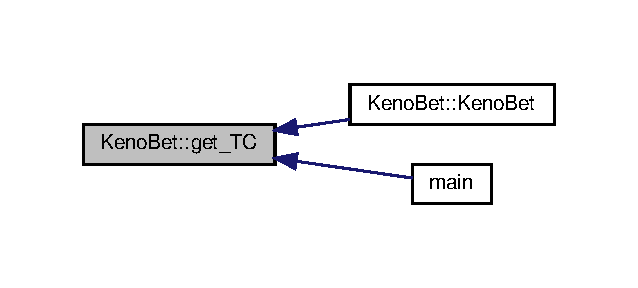
\includegraphics[width=306pt]{classKenoBet_ade294f6dcb57c7a55be5ce2303664b0a_icgraph}
\end{center}
\end{figure}
\mbox{\Hypertarget{classKenoBet_a15782d60d2e9b76f359963865a714a04}\label{classKenoBet_a15782d60d2e9b76f359963865a714a04}} 
\index{Keno\+Bet@{Keno\+Bet}!get\+\_\+\+T\+SC@{get\+\_\+\+T\+SC}}
\index{get\+\_\+\+T\+SC@{get\+\_\+\+T\+SC}!Keno\+Bet@{Keno\+Bet}}
\subsubsection{\texorpdfstring{get\+\_\+\+T\+S\+C()}{get\_TSC()}}
{\footnotesize\ttfamily float Keno\+Bet\+::get\+\_\+\+T\+SC (\begin{DoxyParamCaption}\item[{void}]{ }\end{DoxyParamCaption}) const}



Get Total Inital Cash. 

\begin{DoxyReturn}{Returns}
Valor of Total Inital Cash. 
\end{DoxyReturn}

\begin{DoxyCode}
123 \{
124     \textcolor{keywordflow}{return} m\_TSC;
125 \}
\end{DoxyCode}
Here is the caller graph for this function\+:
\nopagebreak
\begin{figure}[H]
\begin{center}
\leavevmode
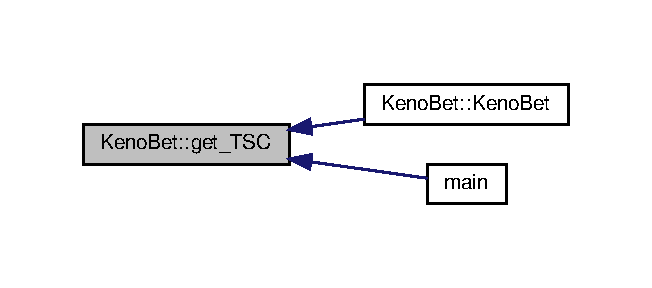
\includegraphics[width=313pt]{classKenoBet_a15782d60d2e9b76f359963865a714a04_icgraph}
\end{center}
\end{figure}
\mbox{\Hypertarget{classKenoBet_a65f0348e49dd8a2e2dddfcc9a1f05a65}\label{classKenoBet_a65f0348e49dd8a2e2dddfcc9a1f05a65}} 
\index{Keno\+Bet@{Keno\+Bet}!get\+\_\+wage@{get\+\_\+wage}}
\index{get\+\_\+wage@{get\+\_\+wage}!Keno\+Bet@{Keno\+Bet}}
\subsubsection{\texorpdfstring{get\+\_\+wage()}{get\_wage()}}
{\footnotesize\ttfamily float Keno\+Bet\+::get\+\_\+wage (\begin{DoxyParamCaption}\item[{void}]{ }\end{DoxyParamCaption}) const}



Retrieves the player ’s wage on this bet . 

\begin{DoxyReturn}{Returns}
The wage value . 
\end{DoxyReturn}
Here is the caller graph for this function\+:
\nopagebreak
\begin{figure}[H]
\begin{center}
\leavevmode
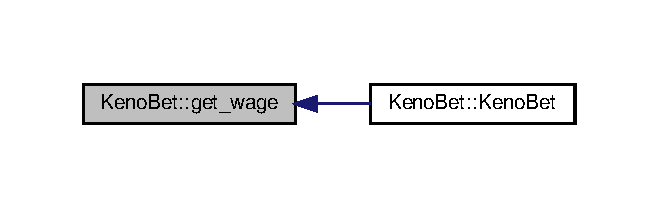
\includegraphics[width=316pt]{classKenoBet_a65f0348e49dd8a2e2dddfcc9a1f05a65_icgraph}
\end{center}
\end{figure}
\mbox{\Hypertarget{classKenoBet_aa2093fa2b053cf74e95d1e6b54d748f3}\label{classKenoBet_aa2093fa2b053cf74e95d1e6b54d748f3}} 
\index{Keno\+Bet@{Keno\+Bet}!hits\+\_\+rdn@{hits\+\_\+rdn}}
\index{hits\+\_\+rdn@{hits\+\_\+rdn}!Keno\+Bet@{Keno\+Bet}}
\subsubsection{\texorpdfstring{hits\+\_\+rdn()}{hits\_rdn()}}
{\footnotesize\ttfamily void Keno\+Bet\+::hits\+\_\+rdn (\begin{DoxyParamCaption}\item[{void}]{ }\end{DoxyParamCaption})}



Randon Hits. 

Here is the caller graph for this function\+:
\nopagebreak
\begin{figure}[H]
\begin{center}
\leavevmode
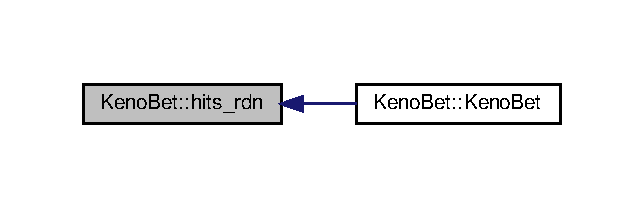
\includegraphics[width=309pt]{classKenoBet_aa2093fa2b053cf74e95d1e6b54d748f3_icgraph}
\end{center}
\end{figure}
\mbox{\Hypertarget{classKenoBet_a5a544a0c1ba5872076e7bfdf8f935368}\label{classKenoBet_a5a544a0c1ba5872076e7bfdf8f935368}} 
\index{Keno\+Bet@{Keno\+Bet}!operator\mbox{[}\mbox{]}@{operator[]}}
\index{operator\mbox{[}\mbox{]}@{operator[]}!Keno\+Bet@{Keno\+Bet}}
\subsubsection{\texorpdfstring{operator[]()}{operator[]()}}
{\footnotesize\ttfamily unsigned int Keno\+Bet\+::operator\mbox{[}$\,$\mbox{]} (\begin{DoxyParamCaption}\item[{int}]{n }\end{DoxyParamCaption})\hspace{0.3cm}{\ttfamily [inline]}}



operator\mbox{[}\mbox{]} 

/param n Index of Vector /return valor of vector 
\begin{DoxyCode}
132         \{
133             \textcolor{keywordflow}{if}(n < 0 || n >= 15)
134             \{
135                 std::cout << \textcolor{stringliteral}{"\(\backslash\)nIndice excede o valor maximo"};
136                 exit(1);
137             \}
138             \textcolor{keywordflow}{return} *(m\_spots.begin()+n);
139         \}
\end{DoxyCode}
Here is the call graph for this function\+:
\nopagebreak
\begin{figure}[H]
\begin{center}
\leavevmode
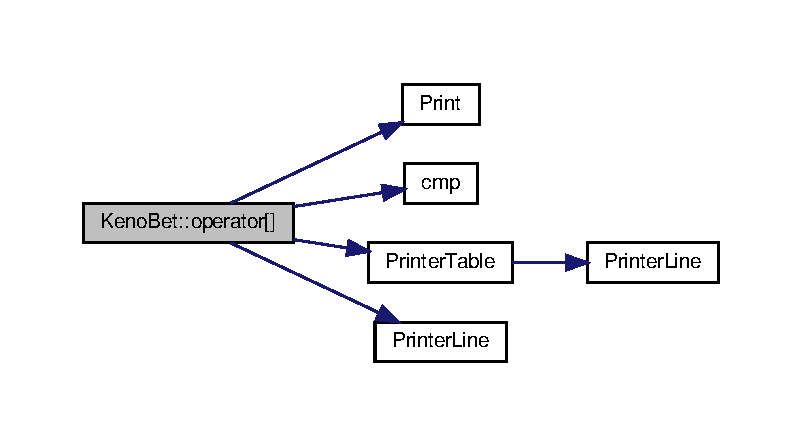
\includegraphics[width=350pt]{classKenoBet_a5a544a0c1ba5872076e7bfdf8f935368_cgraph}
\end{center}
\end{figure}
\mbox{\Hypertarget{classKenoBet_acc2afd4d502e44fdfbb122f3389bc633}\label{classKenoBet_acc2afd4d502e44fdfbb122f3389bc633}} 
\index{Keno\+Bet@{Keno\+Bet}!reset@{reset}}
\index{reset@{reset}!Keno\+Bet@{Keno\+Bet}}
\subsubsection{\texorpdfstring{reset()}{reset()}}
{\footnotesize\ttfamily void Keno\+Bet\+::reset (\begin{DoxyParamCaption}\item[{void}]{ }\end{DoxyParamCaption})}



! Resets a bet to an empty state. 


\begin{DoxyCode}
174 \{   
175     \textcolor{keywordflow}{while}( m\_spots\_r.begin() != m\_spots\_r.end() )
176         m\_spots\_r.pop\_back();
177     \textcolor{keywordflow}{while}( m\_spots.begin() != m\_spots.end() )
178         m\_spots.pop\_back();
179     \textcolor{keywordflow}{while}( m\_spots\_rdn.begin() != m\_spots\_rdn.end() )
180         m\_spots\_rdn.pop\_back();
181     m\_spots\_h = 0;
182 \}
\end{DoxyCode}
Here is the caller graph for this function\+:
\nopagebreak
\begin{figure}[H]
\begin{center}
\leavevmode
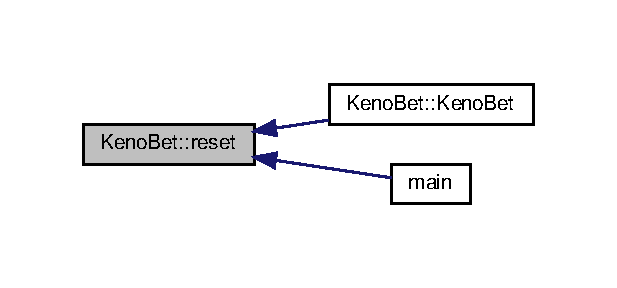
\includegraphics[width=296pt]{classKenoBet_acc2afd4d502e44fdfbb122f3389bc633_icgraph}
\end{center}
\end{figure}
\mbox{\Hypertarget{classKenoBet_a7b74641d226e6b2ea45bc60889f32781}\label{classKenoBet_a7b74641d226e6b2ea45bc60889f32781}} 
\index{Keno\+Bet@{Keno\+Bet}!set\+\_\+\+IC@{set\+\_\+\+IC}}
\index{set\+\_\+\+IC@{set\+\_\+\+IC}!Keno\+Bet@{Keno\+Bet}}
\subsubsection{\texorpdfstring{set\+\_\+\+I\+C()}{set\_IC()}}
{\footnotesize\ttfamily void Keno\+Bet\+::set\+\_\+\+IC (\begin{DoxyParamCaption}\item[{const float \&}]{n\+\_\+\+IC }\end{DoxyParamCaption})}



!\+Set Inital Cash. 


\begin{DoxyCode}
131 \{
132     m\_IC = n\_IC;
133 \}
\end{DoxyCode}
Here is the caller graph for this function\+:
\nopagebreak
\begin{figure}[H]
\begin{center}
\leavevmode
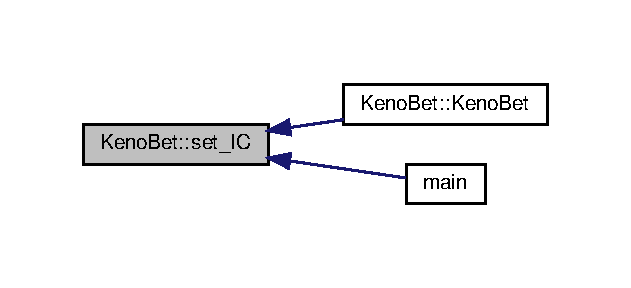
\includegraphics[width=303pt]{classKenoBet_a7b74641d226e6b2ea45bc60889f32781_icgraph}
\end{center}
\end{figure}
\mbox{\Hypertarget{classKenoBet_a63780c5d19157760a2760407cd68149f}\label{classKenoBet_a63780c5d19157760a2760407cd68149f}} 
\index{Keno\+Bet@{Keno\+Bet}!set\+\_\+\+NR@{set\+\_\+\+NR}}
\index{set\+\_\+\+NR@{set\+\_\+\+NR}!Keno\+Bet@{Keno\+Bet}}
\subsubsection{\texorpdfstring{set\+\_\+\+N\+R()}{set\_NR()}}
{\footnotesize\ttfamily void Keno\+Bet\+::set\+\_\+\+NR (\begin{DoxyParamCaption}\item[{const int \&}]{n\+\_\+\+NR }\end{DoxyParamCaption})}



!\+Set Numbers Rounds. 


\begin{DoxyCode}
147 \{
148     m\_NR = n\_NR;
149 \}
\end{DoxyCode}
Here is the caller graph for this function\+:
\nopagebreak
\begin{figure}[H]
\begin{center}
\leavevmode
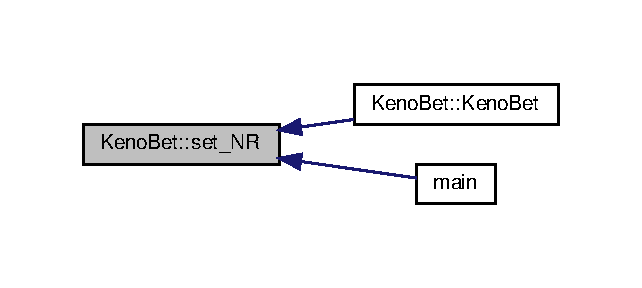
\includegraphics[width=308pt]{classKenoBet_a63780c5d19157760a2760407cd68149f_icgraph}
\end{center}
\end{figure}
\mbox{\Hypertarget{classKenoBet_a4865fd866acc1500bde749d8d15ddf16}\label{classKenoBet_a4865fd866acc1500bde749d8d15ddf16}} 
\index{Keno\+Bet@{Keno\+Bet}!set\+\_\+\+SC@{set\+\_\+\+SC}}
\index{set\+\_\+\+SC@{set\+\_\+\+SC}!Keno\+Bet@{Keno\+Bet}}
\subsubsection{\texorpdfstring{set\+\_\+\+S\+C()}{set\_SC()}}
{\footnotesize\ttfamily void Keno\+Bet\+::set\+\_\+\+SC (\begin{DoxyParamCaption}\item[{const float \&}]{n\+\_\+\+SC }\end{DoxyParamCaption})}



!\+Set Spend Cash per round. 


\begin{DoxyCode}
139 \{
140     m\_SC = n\_SC;
141 \}
\end{DoxyCode}
Here is the caller graph for this function\+:
\nopagebreak
\begin{figure}[H]
\begin{center}
\leavevmode
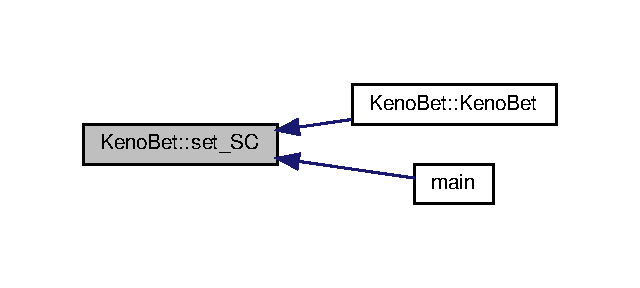
\includegraphics[width=307pt]{classKenoBet_a4865fd866acc1500bde749d8d15ddf16_icgraph}
\end{center}
\end{figure}
\mbox{\Hypertarget{classKenoBet_acdeff501accf00661e0151901bc888c0}\label{classKenoBet_acdeff501accf00661e0151901bc888c0}} 
\index{Keno\+Bet@{Keno\+Bet}!set\+\_\+spot\+\_\+h@{set\+\_\+spot\+\_\+h}}
\index{set\+\_\+spot\+\_\+h@{set\+\_\+spot\+\_\+h}!Keno\+Bet@{Keno\+Bet}}
\subsubsection{\texorpdfstring{set\+\_\+spot\+\_\+h()}{set\_spot\_h()}}
{\footnotesize\ttfamily void Keno\+Bet\+::set\+\_\+spot\+\_\+h (\begin{DoxyParamCaption}\item[{int}]{n\+\_\+spot\+\_\+r }\end{DoxyParamCaption})}



!\+Set valor of hits right. 


\begin{DoxyCode}
151 \{
152     m\_spots\_h = n\_spot\_r; 
153 \}
\end{DoxyCode}
Here is the caller graph for this function\+:
\nopagebreak
\begin{figure}[H]
\begin{center}
\leavevmode
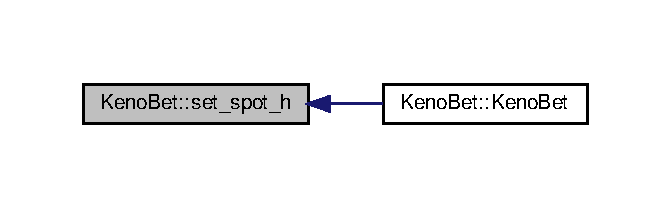
\includegraphics[width=322pt]{classKenoBet_acdeff501accf00661e0151901bc888c0_icgraph}
\end{center}
\end{figure}
\mbox{\Hypertarget{classKenoBet_aa9be1ef95a09fcc293e7c73e763ff176}\label{classKenoBet_aa9be1ef95a09fcc293e7c73e763ff176}} 
\index{Keno\+Bet@{Keno\+Bet}!set\+\_\+\+TC@{set\+\_\+\+TC}}
\index{set\+\_\+\+TC@{set\+\_\+\+TC}!Keno\+Bet@{Keno\+Bet}}
\subsubsection{\texorpdfstring{set\+\_\+\+T\+C()}{set\_TC()}}
{\footnotesize\ttfamily void Keno\+Bet\+::set\+\_\+\+TC (\begin{DoxyParamCaption}\item[{const float \&}]{n\+\_\+\+TC }\end{DoxyParamCaption})}



!\+Set Total Cash 


\begin{DoxyCode}
135 \{
136     m\_TC = n\_TC;
137 \}
\end{DoxyCode}
Here is the caller graph for this function\+:
\nopagebreak
\begin{figure}[H]
\begin{center}
\leavevmode
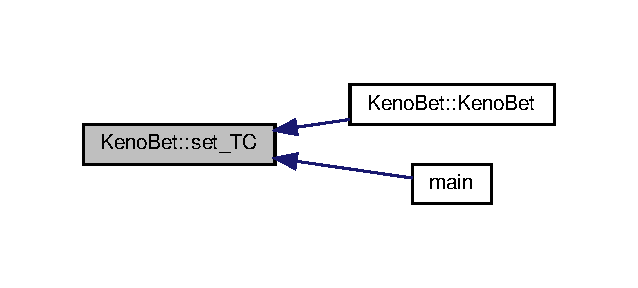
\includegraphics[width=306pt]{classKenoBet_aa9be1ef95a09fcc293e7c73e763ff176_icgraph}
\end{center}
\end{figure}
\mbox{\Hypertarget{classKenoBet_abd6b6b0b0ed9c3d030a71673dc89f39a}\label{classKenoBet_abd6b6b0b0ed9c3d030a71673dc89f39a}} 
\index{Keno\+Bet@{Keno\+Bet}!set\+\_\+\+T\+SC@{set\+\_\+\+T\+SC}}
\index{set\+\_\+\+T\+SC@{set\+\_\+\+T\+SC}!Keno\+Bet@{Keno\+Bet}}
\subsubsection{\texorpdfstring{set\+\_\+\+T\+S\+C()}{set\_TSC()}}
{\footnotesize\ttfamily void Keno\+Bet\+::set\+\_\+\+T\+SC (\begin{DoxyParamCaption}\item[{const float \&}]{n\+\_\+\+T\+SC }\end{DoxyParamCaption})}



!set Total Spend Cash. 


\begin{DoxyCode}
143 \{
144     m\_TSC = n\_TSC;
145 \}
\end{DoxyCode}
Here is the caller graph for this function\+:
\nopagebreak
\begin{figure}[H]
\begin{center}
\leavevmode
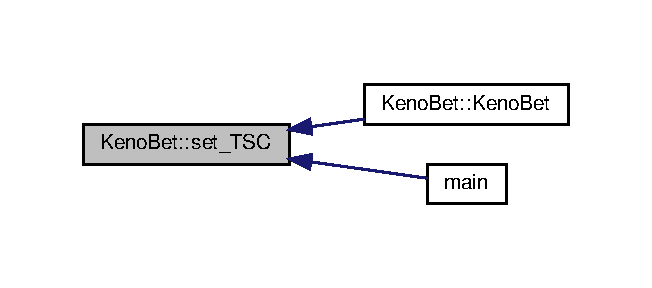
\includegraphics[width=313pt]{classKenoBet_abd6b6b0b0ed9c3d030a71673dc89f39a_icgraph}
\end{center}
\end{figure}
\mbox{\Hypertarget{classKenoBet_a2b21e387cde33818230d9895845b2d9a}\label{classKenoBet_a2b21e387cde33818230d9895845b2d9a}} 
\index{Keno\+Bet@{Keno\+Bet}!set\+\_\+wage@{set\+\_\+wage}}
\index{set\+\_\+wage@{set\+\_\+wage}!Keno\+Bet@{Keno\+Bet}}
\subsubsection{\texorpdfstring{set\+\_\+wage()}{set\_wage()}}
{\footnotesize\ttfamily bool Keno\+Bet\+::set\+\_\+wage (\begin{DoxyParamCaption}\item[{float}]{wage\+\_\+ }\end{DoxyParamCaption})}



Sets the amount of money the player is betting. 


\begin{DoxyParams}{Parameters}
{\em wage\+\_\+} & The wage . \\
\hline
\end{DoxyParams}
\begin{DoxyReturn}{Returns}
True if we have a wage above zero ; false otherwise. 
\end{DoxyReturn}

\begin{DoxyCode}
155 \{
156     \textcolor{keywordflow}{return} m\_IC < 0;
157 \}
\end{DoxyCode}
Here is the caller graph for this function\+:
\nopagebreak
\begin{figure}[H]
\begin{center}
\leavevmode
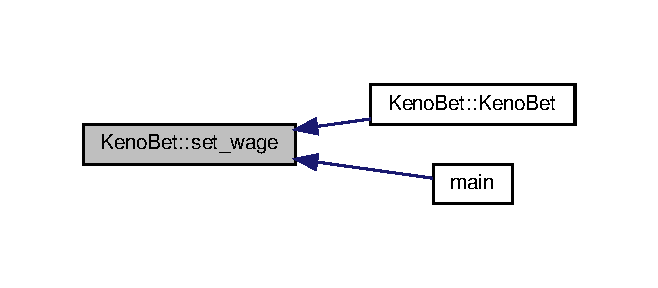
\includegraphics[width=316pt]{classKenoBet_a2b21e387cde33818230d9895845b2d9a_icgraph}
\end{center}
\end{figure}
\mbox{\Hypertarget{classKenoBet_aa6f65b35514270c2707e60b9dea23ae9}\label{classKenoBet_aa6f65b35514270c2707e60b9dea23ae9}} 
\index{Keno\+Bet@{Keno\+Bet}!size@{size}}
\index{size@{size}!Keno\+Bet@{Keno\+Bet}}
\subsubsection{\texorpdfstring{size()}{size()}}
{\footnotesize\ttfamily size\+\_\+t Keno\+Bet\+::size (\begin{DoxyParamCaption}\item[{void}]{ }\end{DoxyParamCaption}) const}



Returns to the current number of spots in the player ’s bet. 

\begin{DoxyReturn}{Returns}
Number of spots present in the bet. 
\end{DoxyReturn}

\begin{DoxyCode}
127 \{
128     \textcolor{keywordflow}{return} m\_NR;
129 \}
\end{DoxyCode}
Here is the caller graph for this function\+:
\nopagebreak
\begin{figure}[H]
\begin{center}
\leavevmode
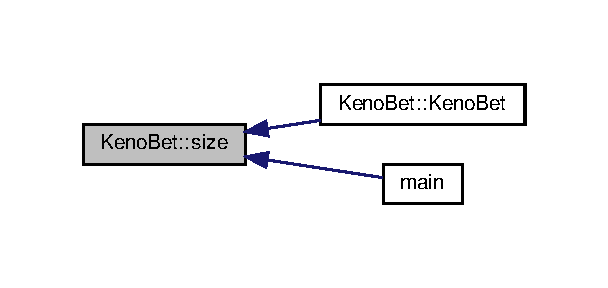
\includegraphics[width=292pt]{classKenoBet_aa6f65b35514270c2707e60b9dea23ae9_icgraph}
\end{center}
\end{figure}


The documentation for this class was generated from the following files\+:\begin{DoxyCompactItemize}
\item 
/home/bergony/lp\+\_\+projeto\+\_\+keno/include/\hyperlink{bet_8h}{bet.\+h}\item 
/home/bergony/lp\+\_\+projeto\+\_\+keno/src/\hyperlink{bet_8cpp}{bet.\+cpp}\end{DoxyCompactItemize}

\chapter{File Documentation}
\hypertarget{bet_8h}{}\section{/home/bergony/lp\+\_\+projeto\+\_\+keno/include/bet.h File Reference}
\label{bet_8h}\index{/home/bergony/lp\+\_\+projeto\+\_\+keno/include/bet.\+h@{/home/bergony/lp\+\_\+projeto\+\_\+keno/include/bet.\+h}}
{\ttfamily \#include $<$iostream$>$}\newline
{\ttfamily \#include $<$stdlib.\+h$>$}\newline
{\ttfamily \#include $<$time.\+h$>$}\newline
{\ttfamily \#include $<$iomanip$>$}\newline
{\ttfamily \#include $<$algorithm$>$}\newline
{\ttfamily \#include $<$vector$>$}\newline
Include dependency graph for bet.\+h\+:
\nopagebreak
\begin{figure}[H]
\begin{center}
\leavevmode
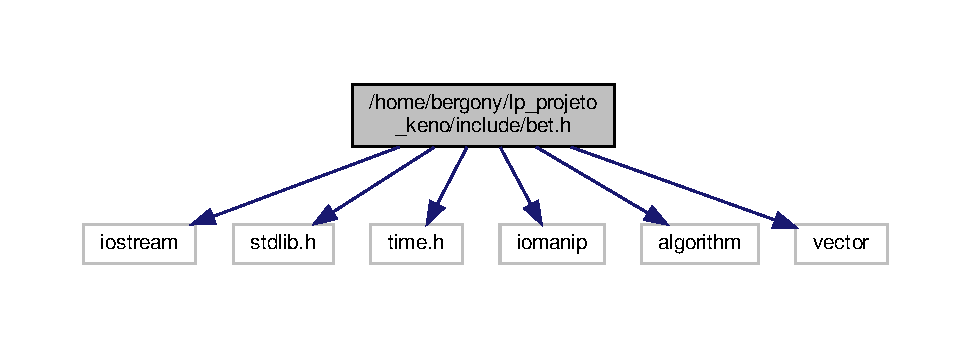
\includegraphics[width=350pt]{bet_8h__incl}
\end{center}
\end{figure}
This graph shows which files directly or indirectly include this file\+:
\nopagebreak
\begin{figure}[H]
\begin{center}
\leavevmode
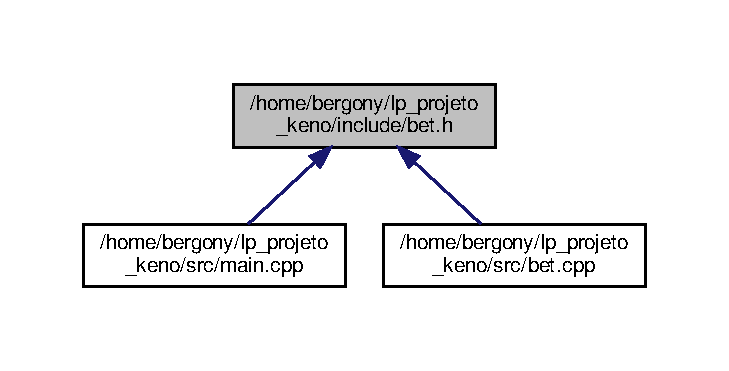
\includegraphics[width=350pt]{bet_8h__dep__incl}
\end{center}
\end{figure}
\subsection*{Classes}
\begin{DoxyCompactItemize}
\item 
class \hyperlink{classKenoBet}{Keno\+Bet}
\end{DoxyCompactItemize}
\subsection*{Functions}
\begin{DoxyCompactItemize}
\item 
void \hyperlink{bet_8h_ae136c90086a2fece05b983a3b7c69401}{Print} (int $\ast$first, int $\ast$last)
\begin{DoxyCompactList}\small\item\em Printer a Vector \mbox{[}x , y) \end{DoxyCompactList}\item 
int \hyperlink{bet_8h_a2e84714d9bda277b7b7d49481189107c}{cmp} (const void $\ast$a, const void $\ast$b)
\begin{DoxyCompactList}\small\item\em Compare two number e and giver if lower equal or lower. \end{DoxyCompactList}\item 
void \hyperlink{bet_8h_aff9e197e7a490d959086fc089c806da7}{Printer\+Table} (void)
\begin{DoxyCompactList}\small\item\em ! Printer Table Payout \end{DoxyCompactList}\item 
void \hyperlink{bet_8h_a2043897413d3ae2277052a1ee9529c18}{Printer\+Line} (int a)
\begin{DoxyCompactList}\small\item\em Pinter line. \end{DoxyCompactList}\end{DoxyCompactItemize}


\subsection{Function Documentation}
\mbox{\Hypertarget{bet_8h_a2e84714d9bda277b7b7d49481189107c}\label{bet_8h_a2e84714d9bda277b7b7d49481189107c}} 
\index{bet.\+h@{bet.\+h}!cmp@{cmp}}
\index{cmp@{cmp}!bet.\+h@{bet.\+h}}
\subsubsection{\texorpdfstring{cmp()}{cmp()}}
{\footnotesize\ttfamily int cmp (\begin{DoxyParamCaption}\item[{const void $\ast$}]{a,  }\item[{const void $\ast$}]{b }\end{DoxyParamCaption})}



Compare two number e and giver if lower equal or lower. 


\begin{DoxyParams}{Parameters}
{\em $\ast$a} & Number 1 . \\
\hline
{\em $\ast$b} & Number 2 . \\
\hline
\end{DoxyParams}
\begin{DoxyReturn}{Returns}
a $<$ b -\/1. 

a = b 0. 

a $>$ b 1. 
\end{DoxyReturn}

\begin{DoxyCode}
4 \{
5     \textcolor{keyword}{const} \textcolor{keywordtype}{int} *cast\_a = (\textcolor{keyword}{const} \textcolor{keywordtype}{int} *)a;
6     \textcolor{keyword}{const} \textcolor{keywordtype}{int} *cast\_b = (\textcolor{keyword}{const} \textcolor{keywordtype}{int} *)b;
7 
8     \textcolor{keywordflow}{if}(*(cast\_a) < *(cast\_b)) 
9         \textcolor{keywordflow}{return} -1;
10     \textcolor{keywordflow}{if}(*(cast\_a) == *(cast\_b)) 
11         \textcolor{keywordflow}{return} 0;
12     \textcolor{keywordflow}{return} 1;
13 \}
\end{DoxyCode}
Here is the caller graph for this function\+:
\nopagebreak
\begin{figure}[H]
\begin{center}
\leavevmode
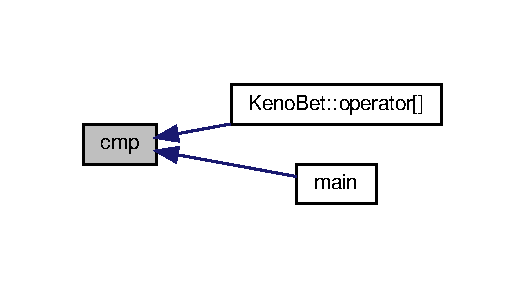
\includegraphics[width=252pt]{bet_8h_a2e84714d9bda277b7b7d49481189107c_icgraph}
\end{center}
\end{figure}
\mbox{\Hypertarget{bet_8h_ae136c90086a2fece05b983a3b7c69401}\label{bet_8h_ae136c90086a2fece05b983a3b7c69401}} 
\index{bet.\+h@{bet.\+h}!Print@{Print}}
\index{Print@{Print}!bet.\+h@{bet.\+h}}
\subsubsection{\texorpdfstring{Print()}{Print()}}
{\footnotesize\ttfamily void Print (\begin{DoxyParamCaption}\item[{int $\ast$}]{first,  }\item[{int $\ast$}]{last }\end{DoxyParamCaption})}



Printer a Vector \mbox{[}x , y) 


\begin{DoxyParams}{Parameters}
{\em $\ast$first} & begin of vector . \\
\hline
{\em $\ast$last} & end of vector . \\
\hline
\end{DoxyParams}

\begin{DoxyCode}
15 \{
16     \textcolor{keyword}{auto} index\{0\};
17     std::cout << \textcolor{stringliteral}{"[ "};
18     \textcolor{keywordflow}{while}( (first+index) != last )
19     \{
20         std::cout << *(first+index) << \textcolor{stringliteral}{" "};
21         index++;
22     \}
23     std::cout << \textcolor{stringliteral}{"]"};
24 \}
\end{DoxyCode}
Here is the caller graph for this function\+:
\nopagebreak
\begin{figure}[H]
\begin{center}
\leavevmode
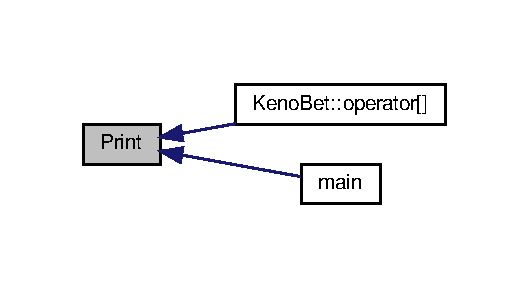
\includegraphics[width=254pt]{bet_8h_ae136c90086a2fece05b983a3b7c69401_icgraph}
\end{center}
\end{figure}
\mbox{\Hypertarget{bet_8h_a2043897413d3ae2277052a1ee9529c18}\label{bet_8h_a2043897413d3ae2277052a1ee9529c18}} 
\index{bet.\+h@{bet.\+h}!Printer\+Line@{Printer\+Line}}
\index{Printer\+Line@{Printer\+Line}!bet.\+h@{bet.\+h}}
\subsubsection{\texorpdfstring{Printer\+Line()}{PrinterLine()}}
{\footnotesize\ttfamily void Printer\+Line (\begin{DoxyParamCaption}\item[{int}]{a }\end{DoxyParamCaption})}



Pinter line. 


\begin{DoxyParams}{Parameters}
{\em a} & Number of Dash \\
\hline
\end{DoxyParams}

\begin{DoxyCode}
26 \{
27     \textcolor{keywordflow}{for}(\textcolor{keywordtype}{int} i\{0\}; i < a; i++)
28         std::cout << \textcolor{stringliteral}{"-"};
29 
30 \}
\end{DoxyCode}
Here is the caller graph for this function\+:
\nopagebreak
\begin{figure}[H]
\begin{center}
\leavevmode
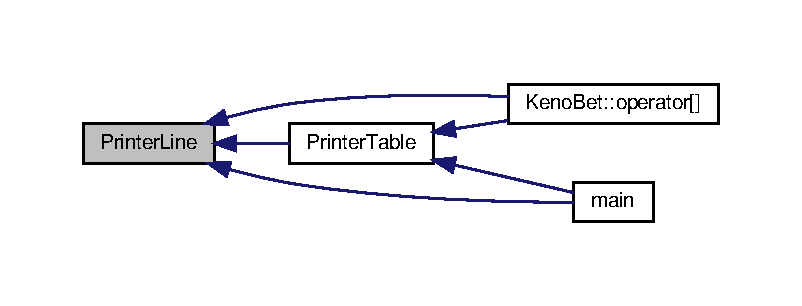
\includegraphics[width=350pt]{bet_8h_a2043897413d3ae2277052a1ee9529c18_icgraph}
\end{center}
\end{figure}
\mbox{\Hypertarget{bet_8h_aff9e197e7a490d959086fc089c806da7}\label{bet_8h_aff9e197e7a490d959086fc089c806da7}} 
\index{bet.\+h@{bet.\+h}!Printer\+Table@{Printer\+Table}}
\index{Printer\+Table@{Printer\+Table}!bet.\+h@{bet.\+h}}
\subsubsection{\texorpdfstring{Printer\+Table()}{PrinterTable()}}
{\footnotesize\ttfamily void Printer\+Table (\begin{DoxyParamCaption}\item[{void}]{ }\end{DoxyParamCaption})}



! Printer Table Payout 


\begin{DoxyCode}
32 \{
33     std::system(\textcolor{stringliteral}{"clear"});
34     std::cout << std::setw(60) << \textcolor{stringliteral}{"hit"} << std::setw(60) << \textcolor{stringliteral}{"\(\backslash\)n"};
35     std::cout << std::setw(15);
36     \hyperlink{bet_8cpp_a2043897413d3ae2277052a1ee9529c18}{PrinterLine}(88);
37     std::cout << \textcolor{stringliteral}{"\(\backslash\)n"};
38     std::cout << \textcolor{stringliteral}{" # spots bet  "};
39     \textcolor{keywordflow}{for}(\textcolor{keywordtype}{int} i\{0\}; i <= 15; i++)
40     \{
41         std::cout << \textcolor{stringliteral}{" "} << i << std::setw(4);
42     \}
43     std::cout << \textcolor{stringliteral}{"\(\backslash\)n"};
44     \hyperlink{bet_8cpp_a2043897413d3ae2277052a1ee9529c18}{PrinterLine}(102);
45     std::cout << \textcolor{stringliteral}{"\(\backslash\)n"};
46     std::cout << std::setw(6) << \textcolor{stringliteral}{"1"} << std::setw(10) << \textcolor{stringliteral}{"0"} << std::setw(5) << \textcolor{stringliteral}{"3"} << std::setw(5)
47         << \textcolor{stringliteral}{"\(\backslash\)n"};
48     std::cout << std::setw(6) << \textcolor{stringliteral}{"2"} << std::setw(10) << \textcolor{stringliteral}{"0"} << std::setw(5) << \textcolor{stringliteral}{"1"} << std::setw(5)
49         << \textcolor{stringliteral}{"9"} << std::setw(5) << \textcolor{stringliteral}{"\(\backslash\)n"};
50     std::cout << std::setw(6) << \textcolor{stringliteral}{"3"} << std::setw(10) << \textcolor{stringliteral}{"0"} << std::setw(5) << \textcolor{stringliteral}{"1"} << std::setw(5)
51         << \textcolor{stringliteral}{"2"} << std::setw(6) << \textcolor{stringliteral}{"16"} << std::setw(5) << \textcolor{stringliteral}{"\(\backslash\)n"};
52     std::cout << std::setw(6) << \textcolor{stringliteral}{"4"} << std::setw(10) << \textcolor{stringliteral}{"0"} << std::setw(6) << \textcolor{stringliteral}{"0.5"} << std::setw(4)
53         << \textcolor{stringliteral}{"2"} << std::setw(5) << \textcolor{stringliteral}{"6"} << std::setw(6) << \textcolor{stringliteral}{"12"} << std::setw(5)
54         << \textcolor{stringliteral}{"\(\backslash\)n"};
55     std::cout << std::setw(6) << \textcolor{stringliteral}{"5"} << std::setw(10)<< \textcolor{stringliteral}{"0"} << std::setw(6) << \textcolor{stringliteral}{"0.5"} << std::setw(4)
56         << \textcolor{stringliteral}{"1"} << std::setw(5) << \textcolor{stringliteral}{"3"} << std::setw(6) << \textcolor{stringliteral}{"15"} << std::setw(5)
57         << \textcolor{stringliteral}{"50"} << std::setw(5) << \textcolor{stringliteral}{"\(\backslash\)n"};
58     std::cout << std::setw(6) << \textcolor{stringliteral}{"6"} <<  std::setw(10)<< \textcolor{stringliteral}{"0"} << std::setw(6) << \textcolor{stringliteral}{"0.5"} << std::setw(4)
59         << \textcolor{stringliteral}{"1"} << std::setw(5) << \textcolor{stringliteral}{"2"} << std::setw(5) << \textcolor{stringliteral}{"3"} << std::setw(6)
60         << \textcolor{stringliteral}{"30"} << std::setw(5) <<  \textcolor{stringliteral}{"75"} << std::setw(5) << \textcolor{stringliteral}{"\(\backslash\)n"};
61     std::cout << std::setw(6) << \textcolor{stringliteral}{"7"} <<  std::setw(10)<< \textcolor{stringliteral}{"0"} << std::setw(6) << \textcolor{stringliteral}{"0.5"} << std::setw(5)
62         << \textcolor{stringliteral}{"0.5"} << std::setw(4) << \textcolor{stringliteral}{"1"} << std::setw(5) << \textcolor{stringliteral}{"6"} << std::setw(6)
63         << \textcolor{stringliteral}{"12"} << std::setw(5) <<  \textcolor{stringliteral}{"36"} << std::setw(5) << \textcolor{stringliteral}{"100"} << std::setw(5)
64         << \textcolor{stringliteral}{"\(\backslash\)n"};
65     std::cout << std::setw(6) << \textcolor{stringliteral}{"8"} <<  std::setw(10)<< \textcolor{stringliteral}{"0"} << std::setw(6) << \textcolor{stringliteral}{"0.5"} << std::setw(5)
66         << \textcolor{stringliteral}{"0.5"} << std::setw(4) << \textcolor{stringliteral}{"1"} << std::setw(5) << \textcolor{stringliteral}{"3"} << std::setw(5)
67         << \textcolor{stringliteral}{"6"} << std::setw(6) << \textcolor{stringliteral}{"19"} << std::setw(4) << \textcolor{stringliteral}{"90"} << std::setw(6)
68         << \textcolor{stringliteral}{"720"} << std::setw(5) << \textcolor{stringliteral}{"\(\backslash\)n"};
69     std::cout << std::setw(6) << \textcolor{stringliteral}{"9"} <<  std::setw(10)<< \textcolor{stringliteral}{"0"} << std::setw(6) << \textcolor{stringliteral}{"0.5"} << std::setw(5)
70         << \textcolor{stringliteral}{"0.5"} << std::setw(4) << \textcolor{stringliteral}{"1"} << std::setw(5) << \textcolor{stringliteral}{"2"} << std::setw(5)
71         << \textcolor{stringliteral}{"4"} << std::setw(5) << \textcolor{stringliteral}{"8"} << std::setw(5) << \textcolor{stringliteral}{"20"} << std::setw(5)
72         << \textcolor{stringliteral}{"80"} << std::setw(7) << \textcolor{stringliteral}{"1200"} << std::setw(5) << \textcolor{stringliteral}{"\(\backslash\)n"};
73     std::cout << std::setw(7) << \textcolor{stringliteral}{"10"} <<  std::setw(9)<< \textcolor{stringliteral}{"0"} << std::setw(5) << \textcolor{stringliteral}{"0"} << std::setw(6)
74         << \textcolor{stringliteral}{"0.5"} << std::setw(4) << \textcolor{stringliteral}{"1"} << std::setw(5) << \textcolor{stringliteral}{"2"} << std::setw(5)
75         << \textcolor{stringliteral}{"3"} << std::setw(5) << \textcolor{stringliteral}{"5"} << std::setw(5) << \textcolor{stringliteral}{"10"} << std::setw(5)
76         << \textcolor{stringliteral}{"30"} << std::setw(6) << \textcolor{stringliteral}{"600"} << std::setw(7) << \textcolor{stringliteral}{"1800"} << std::setw(5)
77         << \textcolor{stringliteral}{"\(\backslash\)n"};
78     std::cout << std::setw(7) << \textcolor{stringliteral}{"11"} <<  std::setw(9)<< \textcolor{stringliteral}{"0"} << std::setw(5) << \textcolor{stringliteral}{"0"} << std::setw(6)
79         << \textcolor{stringliteral}{"0.5"} << std::setw(4) << \textcolor{stringliteral}{"1"} << std::setw(5) << \textcolor{stringliteral}{"1"} << std::setw(5)
80         << \textcolor{stringliteral}{"2"} << std::setw(5) << \textcolor{stringliteral}{"6"} << std::setw(5) << \textcolor{stringliteral}{"15"} << std::setw(5)
81         << \textcolor{stringliteral}{"25"} << std::setw(6) << \textcolor{stringliteral}{"180"} << std::setw(7) << \textcolor{stringliteral}{"1000"} << std::setw(6)
82         << \textcolor{stringliteral}{"3000"} << std::setw(5) <<\textcolor{stringliteral}{"\(\backslash\)n"};
83     std::cout << std::setw(7) << \textcolor{stringliteral}{"12"} <<  std::setw(9)<< \textcolor{stringliteral}{"0"} << std::setw(5) << \textcolor{stringliteral}{"0"} << std::setw(5)
84         << \textcolor{stringliteral}{"0"} << std::setw(6) << \textcolor{stringliteral}{"0.5"} << std::setw(4) << \textcolor{stringliteral}{"1"} << std::setw(5)
85         << \textcolor{stringliteral}{"2"} << std::setw(5) << \textcolor{stringliteral}{"4"} << std::setw(5) << \textcolor{stringliteral}{"24"} << std::setw(5)
86         << \textcolor{stringliteral}{"72"} << std::setw(6) << \textcolor{stringliteral}{"250"} << std::setw(6) << \textcolor{stringliteral}{"500"} << std::setw(7)
87         << \textcolor{stringliteral}{"3000"} << std::setw(6) << \textcolor{stringliteral}{"6000"} << std::setw(5) << \textcolor{stringliteral}{"\(\backslash\)n"};
88     std::cout << std::setw(7) << \textcolor{stringliteral}{"13"} <<  std::setw(9)<< \textcolor{stringliteral}{"0"} << std::setw(5) << \textcolor{stringliteral}{"0"} << std::setw(5)
89         << \textcolor{stringliteral}{"0"} << std::setw(6) << \textcolor{stringliteral}{"0.5"} << std::setw(5) << \textcolor{stringliteral}{"0.5"} << std::setw(4)
90         << \textcolor{stringliteral}{"3"} << std::setw(5) << \textcolor{stringliteral}{"4"} << std::setw(4) << \textcolor{stringliteral}{"5"} << std::setw(6)
91         << \textcolor{stringliteral}{"20"} << std::setw(5) << \textcolor{stringliteral}{"80"} << std::setw(7) << \textcolor{stringliteral}{"240"} << std::setw(6)
92         << \textcolor{stringliteral}{"500"} << std::setw(7) << \textcolor{stringliteral}{"3000"} << std::setw(6) << \textcolor{stringliteral}{"6000"} << std::setw(5)
93         << \textcolor{stringliteral}{"\(\backslash\)n"};
94     std::cout << std::setw(7) << \textcolor{stringliteral}{"14"} <<  std::setw(9)<< \textcolor{stringliteral}{"0"} << std::setw(5) << \textcolor{stringliteral}{"0"} << std::setw(5)
95         << \textcolor{stringliteral}{"0"} << std::setw(6) << \textcolor{stringliteral}{"0.5"} << std::setw(5) << \textcolor{stringliteral}{"0.5"} << std::setw(4)
96         << \textcolor{stringliteral}{"2"} << std::setw(5) << \textcolor{stringliteral}{"3"} << std::setw(4) << \textcolor{stringliteral}{"5"} << std::setw(6)
97         << \textcolor{stringliteral}{"12"} << std::setw(5) << \textcolor{stringliteral}{"50"} << std::setw(7) << \textcolor{stringliteral}{"150"} << std::setw(6)
98         << \textcolor{stringliteral}{"500"} << std::setw(7) << \textcolor{stringliteral}{"1000"} << std::setw(6) << \textcolor{stringliteral}{"2000"} << std::setw(6)
99         << \textcolor{stringliteral}{"7500"} << std::setw(5) << \textcolor{stringliteral}{"\(\backslash\)n"};
100     std::cout << std::setw(7) << \textcolor{stringliteral}{"15"} <<  std::setw(9)<< \textcolor{stringliteral}{"0"} << std::setw(5) << \textcolor{stringliteral}{"0"} << std::setw(5)
101         << \textcolor{stringliteral}{"0"} << std::setw(6) << \textcolor{stringliteral}{"0.5"} << std::setw(5) << \textcolor{stringliteral}{"0.5"} << std::setw(4)
102         << \textcolor{stringliteral}{"1"} << std::setw(5) << \textcolor{stringliteral}{"2"} << std::setw(4) << \textcolor{stringliteral}{"5"} << std::setw(6)
103         << \textcolor{stringliteral}{"15"} << std::setw(5) << \textcolor{stringliteral}{"50"} << std::setw(7) << \textcolor{stringliteral}{"150"} << std::setw(6)
104         << \textcolor{stringliteral}{"300"} << std::setw(6) << \textcolor{stringliteral}{"600"} << std::setw(7) << \textcolor{stringliteral}{"1200"} << std::setw(6)
105         << \textcolor{stringliteral}{"2500"} << std::setw(7) << \textcolor{stringliteral}{"10000"} << std::setw(5) <<\textcolor{stringliteral}{"\(\backslash\)n"};
106 
107     \hyperlink{bet_8cpp_a2043897413d3ae2277052a1ee9529c18}{PrinterLine}(102);
108     std::cout << \textcolor{stringliteral}{"\(\backslash\)n"};
109 \}
\end{DoxyCode}
Here is the call graph for this function\+:
\nopagebreak
\begin{figure}[H]
\begin{center}
\leavevmode
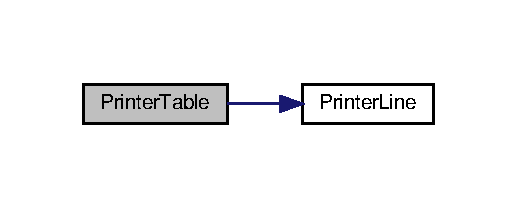
\includegraphics[width=248pt]{bet_8h_aff9e197e7a490d959086fc089c806da7_cgraph}
\end{center}
\end{figure}
Here is the caller graph for this function\+:
\nopagebreak
\begin{figure}[H]
\begin{center}
\leavevmode
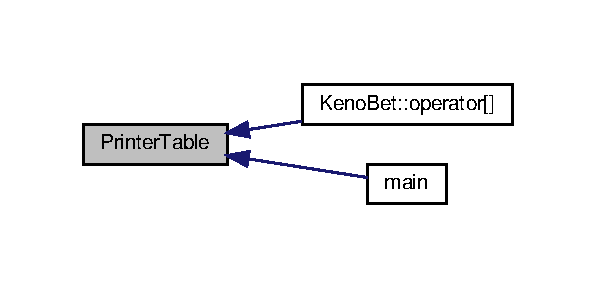
\includegraphics[width=286pt]{bet_8h_aff9e197e7a490d959086fc089c806da7_icgraph}
\end{center}
\end{figure}

\hypertarget{bet_8cpp}{}\section{/home/bergony/lp\+\_\+projeto\+\_\+keno/src/bet.cpp File Reference}
\label{bet_8cpp}\index{/home/bergony/lp\+\_\+projeto\+\_\+keno/src/bet.\+cpp@{/home/bergony/lp\+\_\+projeto\+\_\+keno/src/bet.\+cpp}}
{\ttfamily \#include \char`\"{}../include/bet.\+h\char`\"{}}\newline
Include dependency graph for bet.\+cpp\+:
\nopagebreak
\begin{figure}[H]
\begin{center}
\leavevmode
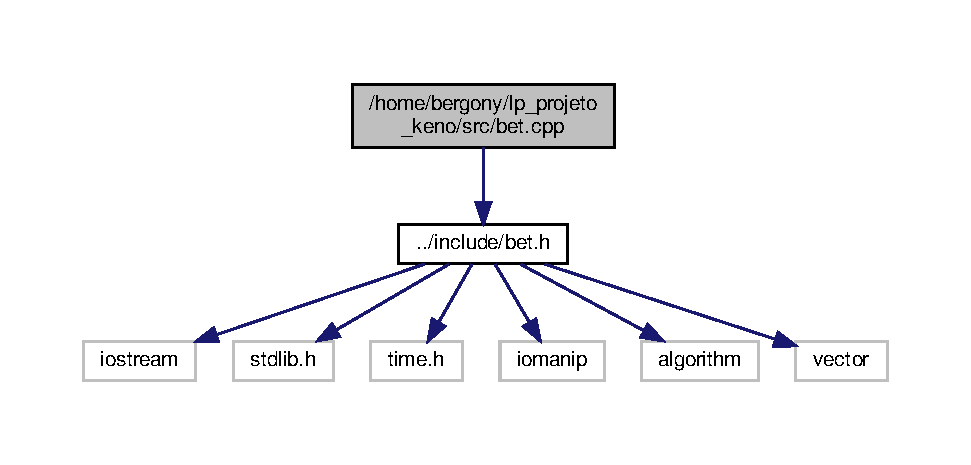
\includegraphics[width=350pt]{bet_8cpp__incl}
\end{center}
\end{figure}
\subsection*{Functions}
\begin{DoxyCompactItemize}
\item 
int \hyperlink{bet_8cpp_a2e84714d9bda277b7b7d49481189107c}{cmp} (const void $\ast$a, const void $\ast$b)
\begin{DoxyCompactList}\small\item\em Compare two number e and giver if lower equal or lower. \end{DoxyCompactList}\item 
void \hyperlink{bet_8cpp_ae136c90086a2fece05b983a3b7c69401}{Print} (int $\ast$first, int $\ast$last)
\begin{DoxyCompactList}\small\item\em Printer a Vector \mbox{[}x , y) \end{DoxyCompactList}\item 
void \hyperlink{bet_8cpp_a2043897413d3ae2277052a1ee9529c18}{Printer\+Line} (int a)
\begin{DoxyCompactList}\small\item\em Pinter line. \end{DoxyCompactList}\item 
void \hyperlink{bet_8cpp_aff9e197e7a490d959086fc089c806da7}{Printer\+Table} (void)
\begin{DoxyCompactList}\small\item\em ! Printer Table Payout \end{DoxyCompactList}\end{DoxyCompactItemize}


\subsection{Function Documentation}
\mbox{\Hypertarget{bet_8cpp_a2e84714d9bda277b7b7d49481189107c}\label{bet_8cpp_a2e84714d9bda277b7b7d49481189107c}} 
\index{bet.\+cpp@{bet.\+cpp}!cmp@{cmp}}
\index{cmp@{cmp}!bet.\+cpp@{bet.\+cpp}}
\subsubsection{\texorpdfstring{cmp()}{cmp()}}
{\footnotesize\ttfamily int cmp (\begin{DoxyParamCaption}\item[{const void $\ast$}]{a,  }\item[{const void $\ast$}]{b }\end{DoxyParamCaption})}



Compare two number e and giver if lower equal or lower. 


\begin{DoxyParams}{Parameters}
{\em $\ast$a} & Number 1 . \\
\hline
{\em $\ast$b} & Number 2 . \\
\hline
\end{DoxyParams}
\begin{DoxyReturn}{Returns}
a $<$ b -\/1. 

a = b 0. 

a $>$ b 1. 
\end{DoxyReturn}

\begin{DoxyCode}
4 \{
5     \textcolor{keyword}{const} \textcolor{keywordtype}{int} *cast\_a = (\textcolor{keyword}{const} \textcolor{keywordtype}{int} *)a;
6     \textcolor{keyword}{const} \textcolor{keywordtype}{int} *cast\_b = (\textcolor{keyword}{const} \textcolor{keywordtype}{int} *)b;
7 
8     \textcolor{keywordflow}{if}(*(cast\_a) < *(cast\_b)) 
9         \textcolor{keywordflow}{return} -1;
10     \textcolor{keywordflow}{if}(*(cast\_a) == *(cast\_b)) 
11         \textcolor{keywordflow}{return} 0;
12     \textcolor{keywordflow}{return} 1;
13 \}
\end{DoxyCode}
Here is the caller graph for this function\+:
\nopagebreak
\begin{figure}[H]
\begin{center}
\leavevmode
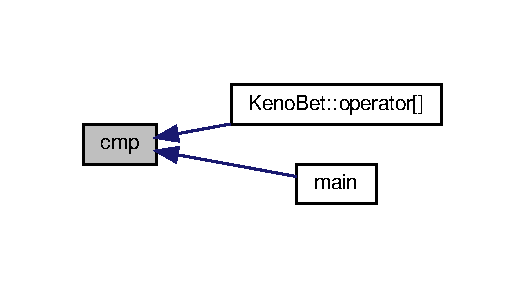
\includegraphics[width=252pt]{bet_8cpp_a2e84714d9bda277b7b7d49481189107c_icgraph}
\end{center}
\end{figure}
\mbox{\Hypertarget{bet_8cpp_ae136c90086a2fece05b983a3b7c69401}\label{bet_8cpp_ae136c90086a2fece05b983a3b7c69401}} 
\index{bet.\+cpp@{bet.\+cpp}!Print@{Print}}
\index{Print@{Print}!bet.\+cpp@{bet.\+cpp}}
\subsubsection{\texorpdfstring{Print()}{Print()}}
{\footnotesize\ttfamily void Print (\begin{DoxyParamCaption}\item[{int $\ast$}]{first,  }\item[{int $\ast$}]{last }\end{DoxyParamCaption})}



Printer a Vector \mbox{[}x , y) 


\begin{DoxyParams}{Parameters}
{\em $\ast$first} & begin of vector . \\
\hline
{\em $\ast$last} & end of vector . \\
\hline
\end{DoxyParams}

\begin{DoxyCode}
15 \{
16     \textcolor{keyword}{auto} index\{0\};
17     std::cout << \textcolor{stringliteral}{"[ "};
18     \textcolor{keywordflow}{while}( (first+index) != last )
19     \{
20         std::cout << *(first+index) << \textcolor{stringliteral}{" "};
21         index++;
22     \}
23     std::cout << \textcolor{stringliteral}{"]"};
24 \}
\end{DoxyCode}
Here is the caller graph for this function\+:
\nopagebreak
\begin{figure}[H]
\begin{center}
\leavevmode
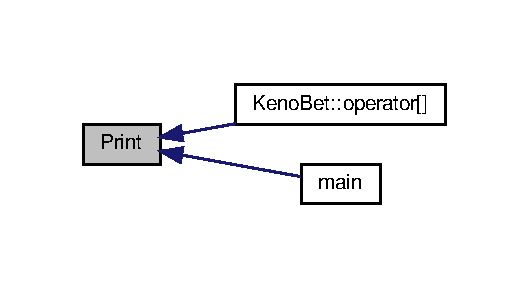
\includegraphics[width=254pt]{bet_8cpp_ae136c90086a2fece05b983a3b7c69401_icgraph}
\end{center}
\end{figure}
\mbox{\Hypertarget{bet_8cpp_a2043897413d3ae2277052a1ee9529c18}\label{bet_8cpp_a2043897413d3ae2277052a1ee9529c18}} 
\index{bet.\+cpp@{bet.\+cpp}!Printer\+Line@{Printer\+Line}}
\index{Printer\+Line@{Printer\+Line}!bet.\+cpp@{bet.\+cpp}}
\subsubsection{\texorpdfstring{Printer\+Line()}{PrinterLine()}}
{\footnotesize\ttfamily void Printer\+Line (\begin{DoxyParamCaption}\item[{int}]{a }\end{DoxyParamCaption})}



Pinter line. 


\begin{DoxyParams}{Parameters}
{\em a} & Number of Dash \\
\hline
\end{DoxyParams}

\begin{DoxyCode}
26 \{
27     \textcolor{keywordflow}{for}(\textcolor{keywordtype}{int} i\{0\}; i < a; i++)
28         std::cout << \textcolor{stringliteral}{"-"};
29 
30 \}
\end{DoxyCode}
Here is the caller graph for this function\+:
\nopagebreak
\begin{figure}[H]
\begin{center}
\leavevmode
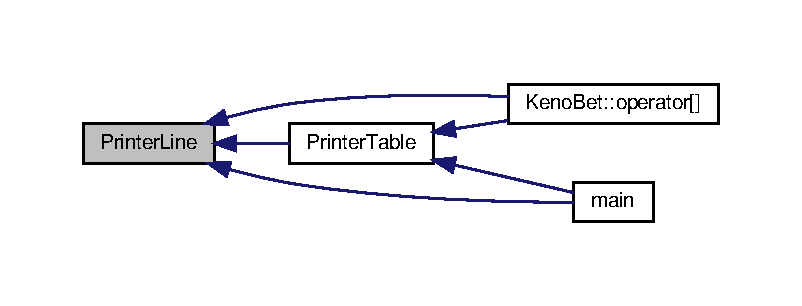
\includegraphics[width=350pt]{bet_8cpp_a2043897413d3ae2277052a1ee9529c18_icgraph}
\end{center}
\end{figure}
\mbox{\Hypertarget{bet_8cpp_aff9e197e7a490d959086fc089c806da7}\label{bet_8cpp_aff9e197e7a490d959086fc089c806da7}} 
\index{bet.\+cpp@{bet.\+cpp}!Printer\+Table@{Printer\+Table}}
\index{Printer\+Table@{Printer\+Table}!bet.\+cpp@{bet.\+cpp}}
\subsubsection{\texorpdfstring{Printer\+Table()}{PrinterTable()}}
{\footnotesize\ttfamily void Printer\+Table (\begin{DoxyParamCaption}\item[{void}]{ }\end{DoxyParamCaption})}



! Printer Table Payout 


\begin{DoxyCode}
32 \{
33     std::system(\textcolor{stringliteral}{"clear"});
34     std::cout << std::setw(60) << \textcolor{stringliteral}{"hit"} << std::setw(60) << \textcolor{stringliteral}{"\(\backslash\)n"};
35     std::cout << std::setw(15);
36     \hyperlink{bet_8cpp_a2043897413d3ae2277052a1ee9529c18}{PrinterLine}(88);
37     std::cout << \textcolor{stringliteral}{"\(\backslash\)n"};
38     std::cout << \textcolor{stringliteral}{" # spots bet  "};
39     \textcolor{keywordflow}{for}(\textcolor{keywordtype}{int} i\{0\}; i <= 15; i++)
40     \{
41         std::cout << \textcolor{stringliteral}{" "} << i << std::setw(4);
42     \}
43     std::cout << \textcolor{stringliteral}{"\(\backslash\)n"};
44     \hyperlink{bet_8cpp_a2043897413d3ae2277052a1ee9529c18}{PrinterLine}(102);
45     std::cout << \textcolor{stringliteral}{"\(\backslash\)n"};
46     std::cout << std::setw(6) << \textcolor{stringliteral}{"1"} << std::setw(10) << \textcolor{stringliteral}{"0"} << std::setw(5) << \textcolor{stringliteral}{"3"} << std::setw(5)
47         << \textcolor{stringliteral}{"\(\backslash\)n"};
48     std::cout << std::setw(6) << \textcolor{stringliteral}{"2"} << std::setw(10) << \textcolor{stringliteral}{"0"} << std::setw(5) << \textcolor{stringliteral}{"1"} << std::setw(5)
49         << \textcolor{stringliteral}{"9"} << std::setw(5) << \textcolor{stringliteral}{"\(\backslash\)n"};
50     std::cout << std::setw(6) << \textcolor{stringliteral}{"3"} << std::setw(10) << \textcolor{stringliteral}{"0"} << std::setw(5) << \textcolor{stringliteral}{"1"} << std::setw(5)
51         << \textcolor{stringliteral}{"2"} << std::setw(6) << \textcolor{stringliteral}{"16"} << std::setw(5) << \textcolor{stringliteral}{"\(\backslash\)n"};
52     std::cout << std::setw(6) << \textcolor{stringliteral}{"4"} << std::setw(10) << \textcolor{stringliteral}{"0"} << std::setw(6) << \textcolor{stringliteral}{"0.5"} << std::setw(4)
53         << \textcolor{stringliteral}{"2"} << std::setw(5) << \textcolor{stringliteral}{"6"} << std::setw(6) << \textcolor{stringliteral}{"12"} << std::setw(5)
54         << \textcolor{stringliteral}{"\(\backslash\)n"};
55     std::cout << std::setw(6) << \textcolor{stringliteral}{"5"} << std::setw(10)<< \textcolor{stringliteral}{"0"} << std::setw(6) << \textcolor{stringliteral}{"0.5"} << std::setw(4)
56         << \textcolor{stringliteral}{"1"} << std::setw(5) << \textcolor{stringliteral}{"3"} << std::setw(6) << \textcolor{stringliteral}{"15"} << std::setw(5)
57         << \textcolor{stringliteral}{"50"} << std::setw(5) << \textcolor{stringliteral}{"\(\backslash\)n"};
58     std::cout << std::setw(6) << \textcolor{stringliteral}{"6"} <<  std::setw(10)<< \textcolor{stringliteral}{"0"} << std::setw(6) << \textcolor{stringliteral}{"0.5"} << std::setw(4)
59         << \textcolor{stringliteral}{"1"} << std::setw(5) << \textcolor{stringliteral}{"2"} << std::setw(5) << \textcolor{stringliteral}{"3"} << std::setw(6)
60         << \textcolor{stringliteral}{"30"} << std::setw(5) <<  \textcolor{stringliteral}{"75"} << std::setw(5) << \textcolor{stringliteral}{"\(\backslash\)n"};
61     std::cout << std::setw(6) << \textcolor{stringliteral}{"7"} <<  std::setw(10)<< \textcolor{stringliteral}{"0"} << std::setw(6) << \textcolor{stringliteral}{"0.5"} << std::setw(5)
62         << \textcolor{stringliteral}{"0.5"} << std::setw(4) << \textcolor{stringliteral}{"1"} << std::setw(5) << \textcolor{stringliteral}{"6"} << std::setw(6)
63         << \textcolor{stringliteral}{"12"} << std::setw(5) <<  \textcolor{stringliteral}{"36"} << std::setw(5) << \textcolor{stringliteral}{"100"} << std::setw(5)
64         << \textcolor{stringliteral}{"\(\backslash\)n"};
65     std::cout << std::setw(6) << \textcolor{stringliteral}{"8"} <<  std::setw(10)<< \textcolor{stringliteral}{"0"} << std::setw(6) << \textcolor{stringliteral}{"0.5"} << std::setw(5)
66         << \textcolor{stringliteral}{"0.5"} << std::setw(4) << \textcolor{stringliteral}{"1"} << std::setw(5) << \textcolor{stringliteral}{"3"} << std::setw(5)
67         << \textcolor{stringliteral}{"6"} << std::setw(6) << \textcolor{stringliteral}{"19"} << std::setw(4) << \textcolor{stringliteral}{"90"} << std::setw(6)
68         << \textcolor{stringliteral}{"720"} << std::setw(5) << \textcolor{stringliteral}{"\(\backslash\)n"};
69     std::cout << std::setw(6) << \textcolor{stringliteral}{"9"} <<  std::setw(10)<< \textcolor{stringliteral}{"0"} << std::setw(6) << \textcolor{stringliteral}{"0.5"} << std::setw(5)
70         << \textcolor{stringliteral}{"0.5"} << std::setw(4) << \textcolor{stringliteral}{"1"} << std::setw(5) << \textcolor{stringliteral}{"2"} << std::setw(5)
71         << \textcolor{stringliteral}{"4"} << std::setw(5) << \textcolor{stringliteral}{"8"} << std::setw(5) << \textcolor{stringliteral}{"20"} << std::setw(5)
72         << \textcolor{stringliteral}{"80"} << std::setw(7) << \textcolor{stringliteral}{"1200"} << std::setw(5) << \textcolor{stringliteral}{"\(\backslash\)n"};
73     std::cout << std::setw(7) << \textcolor{stringliteral}{"10"} <<  std::setw(9)<< \textcolor{stringliteral}{"0"} << std::setw(5) << \textcolor{stringliteral}{"0"} << std::setw(6)
74         << \textcolor{stringliteral}{"0.5"} << std::setw(4) << \textcolor{stringliteral}{"1"} << std::setw(5) << \textcolor{stringliteral}{"2"} << std::setw(5)
75         << \textcolor{stringliteral}{"3"} << std::setw(5) << \textcolor{stringliteral}{"5"} << std::setw(5) << \textcolor{stringliteral}{"10"} << std::setw(5)
76         << \textcolor{stringliteral}{"30"} << std::setw(6) << \textcolor{stringliteral}{"600"} << std::setw(7) << \textcolor{stringliteral}{"1800"} << std::setw(5)
77         << \textcolor{stringliteral}{"\(\backslash\)n"};
78     std::cout << std::setw(7) << \textcolor{stringliteral}{"11"} <<  std::setw(9)<< \textcolor{stringliteral}{"0"} << std::setw(5) << \textcolor{stringliteral}{"0"} << std::setw(6)
79         << \textcolor{stringliteral}{"0.5"} << std::setw(4) << \textcolor{stringliteral}{"1"} << std::setw(5) << \textcolor{stringliteral}{"1"} << std::setw(5)
80         << \textcolor{stringliteral}{"2"} << std::setw(5) << \textcolor{stringliteral}{"6"} << std::setw(5) << \textcolor{stringliteral}{"15"} << std::setw(5)
81         << \textcolor{stringliteral}{"25"} << std::setw(6) << \textcolor{stringliteral}{"180"} << std::setw(7) << \textcolor{stringliteral}{"1000"} << std::setw(6)
82         << \textcolor{stringliteral}{"3000"} << std::setw(5) <<\textcolor{stringliteral}{"\(\backslash\)n"};
83     std::cout << std::setw(7) << \textcolor{stringliteral}{"12"} <<  std::setw(9)<< \textcolor{stringliteral}{"0"} << std::setw(5) << \textcolor{stringliteral}{"0"} << std::setw(5)
84         << \textcolor{stringliteral}{"0"} << std::setw(6) << \textcolor{stringliteral}{"0.5"} << std::setw(4) << \textcolor{stringliteral}{"1"} << std::setw(5)
85         << \textcolor{stringliteral}{"2"} << std::setw(5) << \textcolor{stringliteral}{"4"} << std::setw(5) << \textcolor{stringliteral}{"24"} << std::setw(5)
86         << \textcolor{stringliteral}{"72"} << std::setw(6) << \textcolor{stringliteral}{"250"} << std::setw(6) << \textcolor{stringliteral}{"500"} << std::setw(7)
87         << \textcolor{stringliteral}{"3000"} << std::setw(6) << \textcolor{stringliteral}{"6000"} << std::setw(5) << \textcolor{stringliteral}{"\(\backslash\)n"};
88     std::cout << std::setw(7) << \textcolor{stringliteral}{"13"} <<  std::setw(9)<< \textcolor{stringliteral}{"0"} << std::setw(5) << \textcolor{stringliteral}{"0"} << std::setw(5)
89         << \textcolor{stringliteral}{"0"} << std::setw(6) << \textcolor{stringliteral}{"0.5"} << std::setw(5) << \textcolor{stringliteral}{"0.5"} << std::setw(4)
90         << \textcolor{stringliteral}{"3"} << std::setw(5) << \textcolor{stringliteral}{"4"} << std::setw(4) << \textcolor{stringliteral}{"5"} << std::setw(6)
91         << \textcolor{stringliteral}{"20"} << std::setw(5) << \textcolor{stringliteral}{"80"} << std::setw(7) << \textcolor{stringliteral}{"240"} << std::setw(6)
92         << \textcolor{stringliteral}{"500"} << std::setw(7) << \textcolor{stringliteral}{"3000"} << std::setw(6) << \textcolor{stringliteral}{"6000"} << std::setw(5)
93         << \textcolor{stringliteral}{"\(\backslash\)n"};
94     std::cout << std::setw(7) << \textcolor{stringliteral}{"14"} <<  std::setw(9)<< \textcolor{stringliteral}{"0"} << std::setw(5) << \textcolor{stringliteral}{"0"} << std::setw(5)
95         << \textcolor{stringliteral}{"0"} << std::setw(6) << \textcolor{stringliteral}{"0.5"} << std::setw(5) << \textcolor{stringliteral}{"0.5"} << std::setw(4)
96         << \textcolor{stringliteral}{"2"} << std::setw(5) << \textcolor{stringliteral}{"3"} << std::setw(4) << \textcolor{stringliteral}{"5"} << std::setw(6)
97         << \textcolor{stringliteral}{"12"} << std::setw(5) << \textcolor{stringliteral}{"50"} << std::setw(7) << \textcolor{stringliteral}{"150"} << std::setw(6)
98         << \textcolor{stringliteral}{"500"} << std::setw(7) << \textcolor{stringliteral}{"1000"} << std::setw(6) << \textcolor{stringliteral}{"2000"} << std::setw(6)
99         << \textcolor{stringliteral}{"7500"} << std::setw(5) << \textcolor{stringliteral}{"\(\backslash\)n"};
100     std::cout << std::setw(7) << \textcolor{stringliteral}{"15"} <<  std::setw(9)<< \textcolor{stringliteral}{"0"} << std::setw(5) << \textcolor{stringliteral}{"0"} << std::setw(5)
101         << \textcolor{stringliteral}{"0"} << std::setw(6) << \textcolor{stringliteral}{"0.5"} << std::setw(5) << \textcolor{stringliteral}{"0.5"} << std::setw(4)
102         << \textcolor{stringliteral}{"1"} << std::setw(5) << \textcolor{stringliteral}{"2"} << std::setw(4) << \textcolor{stringliteral}{"5"} << std::setw(6)
103         << \textcolor{stringliteral}{"15"} << std::setw(5) << \textcolor{stringliteral}{"50"} << std::setw(7) << \textcolor{stringliteral}{"150"} << std::setw(6)
104         << \textcolor{stringliteral}{"300"} << std::setw(6) << \textcolor{stringliteral}{"600"} << std::setw(7) << \textcolor{stringliteral}{"1200"} << std::setw(6)
105         << \textcolor{stringliteral}{"2500"} << std::setw(7) << \textcolor{stringliteral}{"10000"} << std::setw(5) <<\textcolor{stringliteral}{"\(\backslash\)n"};
106 
107     \hyperlink{bet_8cpp_a2043897413d3ae2277052a1ee9529c18}{PrinterLine}(102);
108     std::cout << \textcolor{stringliteral}{"\(\backslash\)n"};
109 \}
\end{DoxyCode}
Here is the call graph for this function\+:
\nopagebreak
\begin{figure}[H]
\begin{center}
\leavevmode
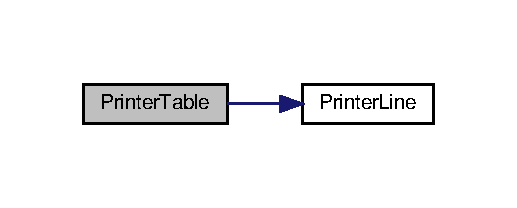
\includegraphics[width=248pt]{bet_8cpp_aff9e197e7a490d959086fc089c806da7_cgraph}
\end{center}
\end{figure}
Here is the caller graph for this function\+:
\nopagebreak
\begin{figure}[H]
\begin{center}
\leavevmode
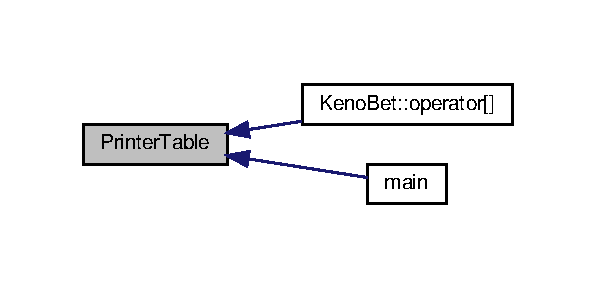
\includegraphics[width=286pt]{bet_8cpp_aff9e197e7a490d959086fc089c806da7_icgraph}
\end{center}
\end{figure}

\hypertarget{main_8cpp}{}\section{/home/bergony/lp\+\_\+projeto\+\_\+keno/src/main.cpp File Reference}
\label{main_8cpp}\index{/home/bergony/lp\+\_\+projeto\+\_\+keno/src/main.\+cpp@{/home/bergony/lp\+\_\+projeto\+\_\+keno/src/main.\+cpp}}
{\ttfamily \#include $<$iostream$>$}\newline
{\ttfamily \#include $<$stdlib.\+h$>$}\newline
{\ttfamily \#include $<$fstream$>$}\newline
{\ttfamily \#include $<$string$>$}\newline
{\ttfamily \#include $<$string.\+h$>$}\newline
{\ttfamily \#include $<$vector$>$}\newline
{\ttfamily \#include \char`\"{}../include/bet.\+h\char`\"{}}\newline
Include dependency graph for main.\+cpp\+:
\nopagebreak
\begin{figure}[H]
\begin{center}
\leavevmode
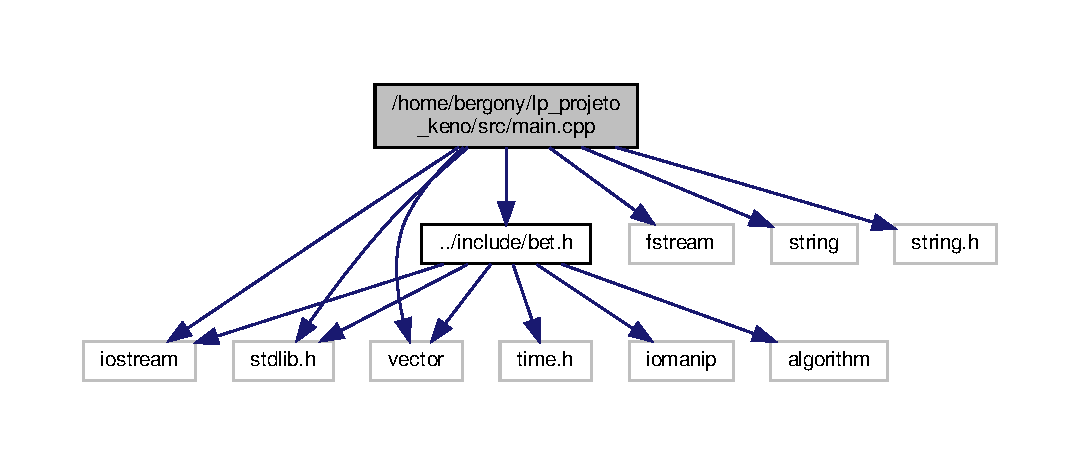
\includegraphics[width=350pt]{main_8cpp__incl}
\end{center}
\end{figure}
\subsection*{Functions}
\begin{DoxyCompactItemize}
\item 
int \hyperlink{main_8cpp_a0ddf1224851353fc92bfbff6f499fa97}{main} (int argc, char $\ast$argv\mbox{[}$\,$\mbox{]})
\end{DoxyCompactItemize}


\subsection{Function Documentation}
\mbox{\Hypertarget{main_8cpp_a0ddf1224851353fc92bfbff6f499fa97}\label{main_8cpp_a0ddf1224851353fc92bfbff6f499fa97}} 
\index{main.\+cpp@{main.\+cpp}!main@{main}}
\index{main@{main}!main.\+cpp@{main.\+cpp}}
\subsubsection{\texorpdfstring{main()}{main()}}
{\footnotesize\ttfamily int main (\begin{DoxyParamCaption}\item[{int}]{argc,  }\item[{char $\ast$}]{argv\mbox{[}$\,$\mbox{]} }\end{DoxyParamCaption})}

This is a \hyperlink{main_8cpp}{main.\+cpp} file here will be

place the bet and full game.

\begin{DoxyAuthor}{Author}
Bergony Bandeira
\end{DoxyAuthor}
\begin{DoxyDate}{Date}
12/10/2018
\end{DoxyDate}

\begin{DoxyCode}
54 \{
55 
57 
66     std::string word;                    \textcolor{comment}{// Word Save string in betfile to be convert.}
67     \textcolor{keywordtype}{char} *bet\_file;                      \textcolor{comment}{// string to save argv[1]}
68     bet\_file = argv[1];
69     std::string::size\_type size\_string;  \textcolor{comment}{// String size}
70     \hyperlink{classKenoBet}{KenoBet} bet;                         \textcolor{comment}{// creates bet objet}
71     \textcolor{keywordtype}{int} endGame\{1\};                      \textcolor{comment}{// Endgame if != 1}
72     \textcolor{keywordtype}{float} *you\_bet;                      \textcolor{comment}{// Arry to save your reward table  bet\_spot\_n}
73 
74     \textcolor{keywordtype}{float} spot\_bet\_1[2] =   \{0,   3\};
75     \textcolor{keywordtype}{float} spot\_bet\_2[3] =   \{0,   1,   9\};
76     \textcolor{keywordtype}{float} spot\_bet\_3[4] =   \{0,   1,   2,  16\};
77     \textcolor{keywordtype}{float} spot\_bet\_4[5] =   \{0, 0.5,   2,   6,  12\};
78     \textcolor{keywordtype}{float} spot\_bet\_5[6] =   \{0, 0.5,   1,   3,  15, 50\};
79     \textcolor{keywordtype}{float} spot\_bet\_6[7] =   \{0, 0.5,   1,   2,   3, 30, 75\};
80     \textcolor{keywordtype}{float} spot\_bet\_7[8] =   \{0, 0.5, 0.5,   1,   6, 12, 36, 100\};
81     \textcolor{keywordtype}{float} spot\_bet\_8[9] =   \{0, 0.5, 0.5,   1,   3,  6, 19,  90, 720\};
82     \textcolor{keywordtype}{float} spot\_bet\_9[10] =  \{0, 0.5, 0.5,   1,   2,  4,  8,  20,  80, 1200\};
83     \textcolor{keywordtype}{float} spot\_bet\_10[11] = \{0,   0, 0.5,   1,   2,  3,  5,  10,  30,  600, 1800\};
84     \textcolor{keywordtype}{float} spot\_bet\_11[12] = \{0,   0, 0.5,   1,   1,  2,  6,  15,  25,  180, 1000, 3000\};
85     \textcolor{keywordtype}{float} spot\_bet\_12[13] = \{0,   0,   0, 0.5,   1,  2,  4,  24,  72,  250,  500, 2000, 4000\};
86     \textcolor{keywordtype}{float} spot\_bet\_13[14] = \{0,   0,   0, 0.5, 0.5,  3,  4,   5,  20,   80,  240,  500, 3000, 6000\};
87     \textcolor{keywordtype}{float} spot\_bet\_14[15] = \{0,   0,   0, 0.5, 0.5,  2,  3,   5,  12,   50,  150,  500, 1000, 2000, 7500\};
88     \textcolor{keywordtype}{float} spot\_bet\_15[16] = \{0,   0,   0, 0.5, 0.5,  1,  2,   5,  15,   50,  150,  300,  600, 1200, 2500, 
      10000\};
89     \textcolor{keywordflow}{while}(endGame == 1)
90     \{
91         std::ifstream fin( bet\_file );                          \textcolor{comment}{//Stream opem in fin}
92 
93         \textcolor{keywordflow}{if} (fin.is\_open())                                      \textcolor{comment}{//if the file is opem}
94         \{
95             getline (fin,word);                                 \textcolor{comment}{//Take the first line}
96             bet.\hyperlink{classKenoBet_a7b74641d226e6b2ea45bc60889f32781}{set\_IC}( std::stof(word, &size\_string));         \textcolor{comment}{//Set initial cash and convert string
       to float}
97             getline (fin,word);                                 \textcolor{comment}{//Take the second line }
98             bet.\hyperlink{classKenoBet_a63780c5d19157760a2760407cd68149f}{set\_NR}( std::stoi(word, &size\_string) );        \textcolor{comment}{//set Number of rounds convert string
       to int}
99             bet.\hyperlink{classKenoBet_abd6b6b0b0ed9c3d030a71673dc89f39a}{set\_TSC}( bet.\hyperlink{classKenoBet_aace00d82c42c9870a4f3b95c7ec79f24}{get\_IC}() );
100             \textcolor{keywordflow}{if}(bet.\hyperlink{classKenoBet_aa6f65b35514270c2707e60b9dea23ae9}{size}() > 15) 
101                 bet.\hyperlink{classKenoBet_a63780c5d19157760a2760407cd68149f}{set\_NR}(15);
102             \hyperlink{bet_8h_aff9e197e7a490d959086fc089c806da7}{PrinterTable}();
103             std::cout << \textcolor{stringliteral}{">>> Preparing to read bet file ["} << argv[1] << \textcolor{stringliteral}{"], please wait...\(\backslash\)n"};
104             \textcolor{keywordflow}{for}(\textcolor{keywordtype}{int} i\{0\}; i < (int)bet.\hyperlink{classKenoBet_aa6f65b35514270c2707e60b9dea23ae9}{size}();i++ )
105             \{
106                 std::getline (fin,word, fin.widen(\textcolor{charliteral}{' '}));                        \textcolor{comment}{//Take the third line up
       until find an blank space.                                            }
107                 \textcolor{keywordflow}{if}(bet.\hyperlink{classKenoBet_aba848a50d30a0155459eb9f5cbb91966}{add\_number}( std::stoi(word, &size\_string) ) == \textcolor{keyword}{false})
108                 \{
109                     std::cout << \textcolor{stringliteral}{"The number is Repeat or the Number of"}
110                               << \textcolor{stringliteral}{"round is high the number of spots"};
111                     \textcolor{keywordflow}{return} -1;
112                 \}
113             \}
114             fin.close();                                        \textcolor{comment}{//Strem close in fin}
115         \}\textcolor{keywordflow}{else}
116         \{
117             std::cerr << \textcolor{stringliteral}{"File is not opem"};
118             \textcolor{keywordflow}{return} -1;
119         \}
120 
121         \textcolor{keywordflow}{if}( bet.\hyperlink{classKenoBet_a2b21e387cde33818230d9895845b2d9a}{set\_wage}( bet.\hyperlink{classKenoBet_aace00d82c42c9870a4f3b95c7ec79f24}{get\_IC}() ) )                                      \textcolor{comment}{//If wage < 0}
122         \{
123             std::cerr << \textcolor{stringliteral}{">>> The Wage initial lower then 0\(\backslash\)n"};
124             \textcolor{keywordflow}{return} -1;
125         \}
126         \textcolor{keywordflow}{if}( bet.\hyperlink{classKenoBet_aa6f65b35514270c2707e60b9dea23ae9}{size}() < 0)                                                     \textcolor{comment}{//Number rounds < 0}
127         \{
128 
129             std::cerr << \textcolor{stringliteral}{">>> The Number Round is lower then 0\(\backslash\)n"};
130             \textcolor{keywordflow}{return} -1;
131         \}
132         \textcolor{keywordflow}{for}(\textcolor{keywordtype}{int} i\{0\}; i < (int)bet.\hyperlink{classKenoBet_aa6f65b35514270c2707e60b9dea23ae9}{size}(); i++)
133         \{
134             \textcolor{keywordflow}{if}(bet[i] > 80 || bet[i] < 1)                                       \textcolor{comment}{//if the spots range (0 80]
        }
135             \{
136                 std::cerr << \textcolor{stringliteral}{"The number is above the 80 or lower then 1\(\backslash\)n"};
137                 \textcolor{keywordflow}{return} -1;
138             \}
139         \}
140         bet.\hyperlink{classKenoBet_a4865fd866acc1500bde749d8d15ddf16}{set\_SC}( bet.\hyperlink{classKenoBet_aace00d82c42c9870a4f3b95c7ec79f24}{get\_IC}()/bet.\hyperlink{classKenoBet_aa6f65b35514270c2707e60b9dea23ae9}{size}());                                              
               \textcolor{comment}{//Set spend cash per round}
141         \hyperlink{bet_8h_a2043897413d3ae2277052a1ee9529c18}{PrinterLine}(58);
142 
143         std::cout << \textcolor{stringliteral}{"\(\backslash\)n>>> Bet successfully read!\(\backslash\)n"};
144         std::cout << \textcolor{stringliteral}{"You are going to wage a total of $"} << bet.\hyperlink{classKenoBet_aace00d82c42c9870a4f3b95c7ec79f24}{get\_IC}() << \textcolor{stringliteral}{" Dollars.\(\backslash\)n"};
145         std::cout << \textcolor{stringliteral}{"Going for a total of "} << bet.\hyperlink{classKenoBet_aa6f65b35514270c2707e60b9dea23ae9}{size}() << \textcolor{stringliteral}{" rounds, waging $"}
146             << bet.\hyperlink{classKenoBet_a0c2ee88fc2f8e7afc5b0399fe74c022b}{get\_SC}() << \textcolor{stringliteral}{" per round.\(\backslash\)n"};
147 
148         you\_bet = \textcolor{keyword}{new} \textcolor{keywordtype}{float}[bet.\hyperlink{classKenoBet_aa6f65b35514270c2707e60b9dea23ae9}{size}()];                                                            \textcolor{comment}{//
      Alloc bet.size to arry reward}
149 
150         \textcolor{keywordflow}{switch} ( bet.\hyperlink{classKenoBet_aa6f65b35514270c2707e60b9dea23ae9}{size}())                                                                        \textcolor{comment}{//
      set reward = number rounds}
151         \{
152             \textcolor{keywordflow}{case} 1 :
153                 you\_bet = spot\_bet\_1;
154                 \textcolor{keywordflow}{break};
155             \textcolor{keywordflow}{case} 2 :
156                 you\_bet = spot\_bet\_2;
157                 \textcolor{keywordflow}{break};
158             \textcolor{keywordflow}{case} 3 :
159                 you\_bet = spot\_bet\_3;
160                 \textcolor{keywordflow}{break};
161             \textcolor{keywordflow}{case} 4 :
162                 you\_bet = spot\_bet\_4;
163                 \textcolor{keywordflow}{break};
164             \textcolor{keywordflow}{case} 5 :
165                 you\_bet = spot\_bet\_5;
166                 \textcolor{keywordflow}{break};
167             \textcolor{keywordflow}{case} 6 :
168                 you\_bet = spot\_bet\_6;
169                 \textcolor{keywordflow}{break};
170             \textcolor{keywordflow}{case} 7 :
171                 you\_bet = spot\_bet\_7;
172                 \textcolor{keywordflow}{break};
173             \textcolor{keywordflow}{case} 8 :
174                 you\_bet = spot\_bet\_8;
175                 \textcolor{keywordflow}{break};
176             \textcolor{keywordflow}{case} 9 :
177                 you\_bet = spot\_bet\_9;
178                 \textcolor{keywordflow}{break};
179             \textcolor{keywordflow}{case} 10 :
180                 you\_bet = spot\_bet\_10;
181                 \textcolor{keywordflow}{break};
182             \textcolor{keywordflow}{case} 11 :
183                 you\_bet = spot\_bet\_11;
184                 \textcolor{keywordflow}{break};
185             \textcolor{keywordflow}{case} 12 :
186                 you\_bet = spot\_bet\_12;
187                 \textcolor{keywordflow}{break};
188             \textcolor{keywordflow}{case} 13 :
189                 you\_bet = spot\_bet\_13;
190                 \textcolor{keywordflow}{break};
191             \textcolor{keywordflow}{case} 14 :
192                 you\_bet = spot\_bet\_14;
193                 \textcolor{keywordflow}{break};
194             default :
195                 you\_bet = spot\_bet\_15;
196         \}
197 
198         std::cout << \textcolor{stringliteral}{"\(\backslash\)nYour bet has "} << bet.\hyperlink{classKenoBet_aa6f65b35514270c2707e60b9dea23ae9}{size}() << \textcolor{stringliteral}{" numbers. They are: "};
199         \hyperlink{bet_8h_ae136c90086a2fece05b983a3b7c69401}{Print}(  bet.\hyperlink{classKenoBet_a386ab5f7108fd2df3518f37bfca2b2ef}{get\_m\_spots}() ,  bet.\hyperlink{classKenoBet_a386ab5f7108fd2df3518f37bfca2b2ef}{get\_m\_spots}()+bet.
      \hyperlink{classKenoBet_aa6f65b35514270c2707e60b9dea23ae9}{size}());
200         std::cout << \textcolor{stringliteral}{"\(\backslash\)n     -------+----------\(\backslash\)n     Hits   | Payout  \(\backslash\)n     -------+----------\(\backslash\)n"} ;
201         \textcolor{keywordflow}{for}(\textcolor{keywordtype}{int} i\{0\}; i <= (int)bet.\hyperlink{classKenoBet_aa6f65b35514270c2707e60b9dea23ae9}{size}(); i++)
202         \{
203             std::cout  << \textcolor{stringliteral}{"     "} << i << \textcolor{stringliteral}{"      |"} << *(you\_bet+i) << \textcolor{stringliteral}{"\(\backslash\)n"};
204         \}
205         std::cout << \textcolor{stringliteral}{"     "};
206         \hyperlink{bet_8h_a2043897413d3ae2277052a1ee9529c18}{PrinterLine}(50);
207         std::cout << \textcolor{stringliteral}{"\(\backslash\)n"};
208         \textcolor{keywordflow}{for}(\textcolor{keywordtype}{int} i\{0\}; i < (int)bet.\hyperlink{classKenoBet_aa6f65b35514270c2707e60b9dea23ae9}{size}(); i++)
209         \{
210             bet.\hyperlink{classKenoBet_a7b74641d226e6b2ea45bc60889f32781}{set\_IC}(bet.\hyperlink{classKenoBet_aace00d82c42c9870a4f3b95c7ec79f24}{get\_IC}() - bet.\hyperlink{classKenoBet_a0c2ee88fc2f8e7afc5b0399fe74c022b}{get\_SC}() );                                    
         \textcolor{comment}{//Pay the bet }
211             std::cout << \textcolor{stringliteral}{"     This is round #"} << i+1 << \textcolor{stringliteral}{" of "} << bet.\hyperlink{classKenoBet_aa6f65b35514270c2707e60b9dea23ae9}{size}()
212                 << \textcolor{stringliteral}{", and your wage is $"} << bet.\hyperlink{classKenoBet_a0c2ee88fc2f8e7afc5b0399fe74c022b}{get\_SC}() << \textcolor{stringliteral}{". Good luck!\(\backslash\)n"};
213             bet.\hyperlink{classKenoBet_a612b57c35203a41682269cdfbb31c2b1}{get\_hits}( bet.\hyperlink{classKenoBet_a382454c66974466900d168c398699483}{get\_spots}() );
214             qsort( bet.\hyperlink{classKenoBet_a8106aa1f149ba3043a8219453e1af3a1}{get\_m\_spots\_rdn}(), 20, \textcolor{keyword}{sizeof}(int), \hyperlink{bet_8h_a2e84714d9bda277b7b7d49481189107c}{cmp});
215             std::cout << \textcolor{stringliteral}{"     The hits are: "};
216             \hyperlink{bet_8h_ae136c90086a2fece05b983a3b7c69401}{Print}( bet.\hyperlink{classKenoBet_a8106aa1f149ba3043a8219453e1af3a1}{get\_m\_spots\_rdn}() , bet.
      \hyperlink{classKenoBet_a8106aa1f149ba3043a8219453e1af3a1}{get\_m\_spots\_rdn}()+20);
217             std::cout << \textcolor{stringliteral}{"\(\backslash\)n"};
218 
219             std::cout << \textcolor{stringliteral}{"\(\backslash\)n     You hit the following number(s) "};
220             \hyperlink{bet_8h_ae136c90086a2fece05b983a3b7c69401}{Print}(  bet.\hyperlink{classKenoBet_a386ab5f7108fd2df3518f37bfca2b2ef}{get\_m\_spots}() ,  bet.\hyperlink{classKenoBet_a386ab5f7108fd2df3518f37bfca2b2ef}{get\_m\_spots}()+bet.
      \hyperlink{classKenoBet_aa6f65b35514270c2707e60b9dea23ae9}{size}());
221 
222             \textcolor{keywordflow}{if}(bet.\hyperlink{classKenoBet_a79f26e472d9a60894e25094a37d06eb6}{get\_spot\_r}() > 0)                                                        \textcolor{comment}{//if
       you get at last one spot}
223                 bet.\hyperlink{classKenoBet_a7b74641d226e6b2ea45bc60889f32781}{set\_IC}( bet.\hyperlink{classKenoBet_aace00d82c42c9870a4f3b95c7ec79f24}{get\_IC}() + ( bet.\hyperlink{classKenoBet_a0c2ee88fc2f8e7afc5b0399fe74c022b}{get\_SC}() * you\_bet[bet.
      \hyperlink{classKenoBet_a79f26e472d9a60894e25094a37d06eb6}{get\_spot\_r}()] ));
224 
225             std::cout << \textcolor{stringliteral}{", a total of "} << bet.\hyperlink{classKenoBet_a79f26e472d9a60894e25094a37d06eb6}{get\_spot\_r}() << \textcolor{stringliteral}{" hits out of "} 
226                 << bet.\hyperlink{classKenoBet_aa6f65b35514270c2707e60b9dea23ae9}{size}() <<\textcolor{stringliteral}{"\(\backslash\)n"} << \textcolor{stringliteral}{"     Payout rate is "} << you\_bet[bet.
      \hyperlink{classKenoBet_a79f26e472d9a60894e25094a37d06eb6}{get\_spot\_r}()] 
227                 << \textcolor{stringliteral}{", thus you came out with: $"} << bet.\hyperlink{classKenoBet_a0c2ee88fc2f8e7afc5b0399fe74c022b}{get\_SC}()*you\_bet[bet.
      \hyperlink{classKenoBet_a79f26e472d9a60894e25094a37d06eb6}{get\_spot\_r}()]
228                 << \textcolor{stringliteral}{"\(\backslash\)n     Your net balance so far is: "} << bet.\hyperlink{classKenoBet_aace00d82c42c9870a4f3b95c7ec79f24}{get\_IC}() << \textcolor{stringliteral}{" Dollars.\(\backslash\)n     "};
229             
230             \hyperlink{bet_8h_a2043897413d3ae2277052a1ee9529c18}{PrinterLine}(50);
231 
232             bet.\hyperlink{classKenoBet_acc2afd4d502e44fdfbb122f3389bc633}{reset}();                                                                    \textcolor{comment}{//reset
       Object Number rounds zero and vector.}
233             std::cin.ignore();
234         \}
235         std::cout<< \textcolor{stringliteral}{">>> End of rounds!\(\backslash\)n"};
236         \hyperlink{bet_8h_a2043897413d3ae2277052a1ee9529c18}{PrinterLine}(58);
237         std::cout << \textcolor{stringliteral}{"\(\backslash\)n \(\backslash\)n===== SUMMARY =====\(\backslash\)n"}
238             << \textcolor{stringliteral}{">>> You spent in this game a total of $"} << bet.\hyperlink{classKenoBet_a15782d60d2e9b76f359963865a714a04}{get\_TSC}() << \textcolor{stringliteral}{" dollars.\(\backslash\)n"};
239         bet.\hyperlink{classKenoBet_aa9be1ef95a09fcc293e7c73e763ff176}{set\_TC}( bet.\hyperlink{classKenoBet_aace00d82c42c9870a4f3b95c7ec79f24}{get\_IC}() - bet.\hyperlink{classKenoBet_a15782d60d2e9b76f359963865a714a04}{get\_TSC}());                                      
           \textcolor{comment}{//Total Cash}
240         \textcolor{keywordflow}{if}(bet.\hyperlink{classKenoBet_ade294f6dcb57c7a55be5ce2303664b0a}{get\_TC}()  > 0)
241         \{
242             std::cout << \textcolor{stringliteral}{">>> Hooray, you won $"} << bet.\hyperlink{classKenoBet_ade294f6dcb57c7a55be5ce2303664b0a}{get\_TC}()
243                       << \textcolor{stringliteral}{" dollars. See you next time! ᕕ( ᐛ )ᕗ"} << std::endl;
244         \}
245         \textcolor{keywordflow}{if}(bet.\hyperlink{classKenoBet_ade294f6dcb57c7a55be5ce2303664b0a}{get\_TC}() < 0)
246         \{
247             std::cout << \textcolor{stringliteral}{">>> Alack, you lost $"} << bet.\hyperlink{classKenoBet_ade294f6dcb57c7a55be5ce2303664b0a}{get\_TC}() 
248                       << \textcolor{stringliteral}{" dollars. See you next time! (⌣̩̩́\_⌣̩̩̀)"} << std::endl;
249         \}
250         \textcolor{keywordflow}{if}(bet.\hyperlink{classKenoBet_ade294f6dcb57c7a55be5ce2303664b0a}{get\_TC}() == 0)
251         \{
252             std::cout << \textcolor{stringliteral}{">>> Whatever, you do not lost $"} << bet.\hyperlink{classKenoBet_ade294f6dcb57c7a55be5ce2303664b0a}{get\_TC}() 
253                       << \textcolor{stringliteral}{" dollars. See you next time! ¯\(\backslash\)\(\backslash\)\_(ツ)\_/¯"} << std::endl;
254         \}
255         std::cout << \textcolor{stringliteral}{">>> You are leaving the Keno table with $"} << bet.\hyperlink{classKenoBet_aace00d82c42c9870a4f3b95c7ec79f24}{get\_IC}() << \textcolor{stringliteral}{" dollars.\(\backslash\)n"};
256         std::cout << \textcolor{stringliteral}{">>> Play Again press 1: "};
257         std::cin >> endGame;
258         \textcolor{keywordflow}{if}(endGame != 1)
259             \textcolor{keywordflow}{break};
260         std::cout << \textcolor{stringliteral}{">>> Enter new data/betn.dat "};
261         std::cin >> bet\_file;
262     \}
263     \textcolor{keywordflow}{return} 0;
264 \}
\end{DoxyCode}
Here is the call graph for this function\+:
\nopagebreak
\begin{figure}[H]
\begin{center}
\leavevmode
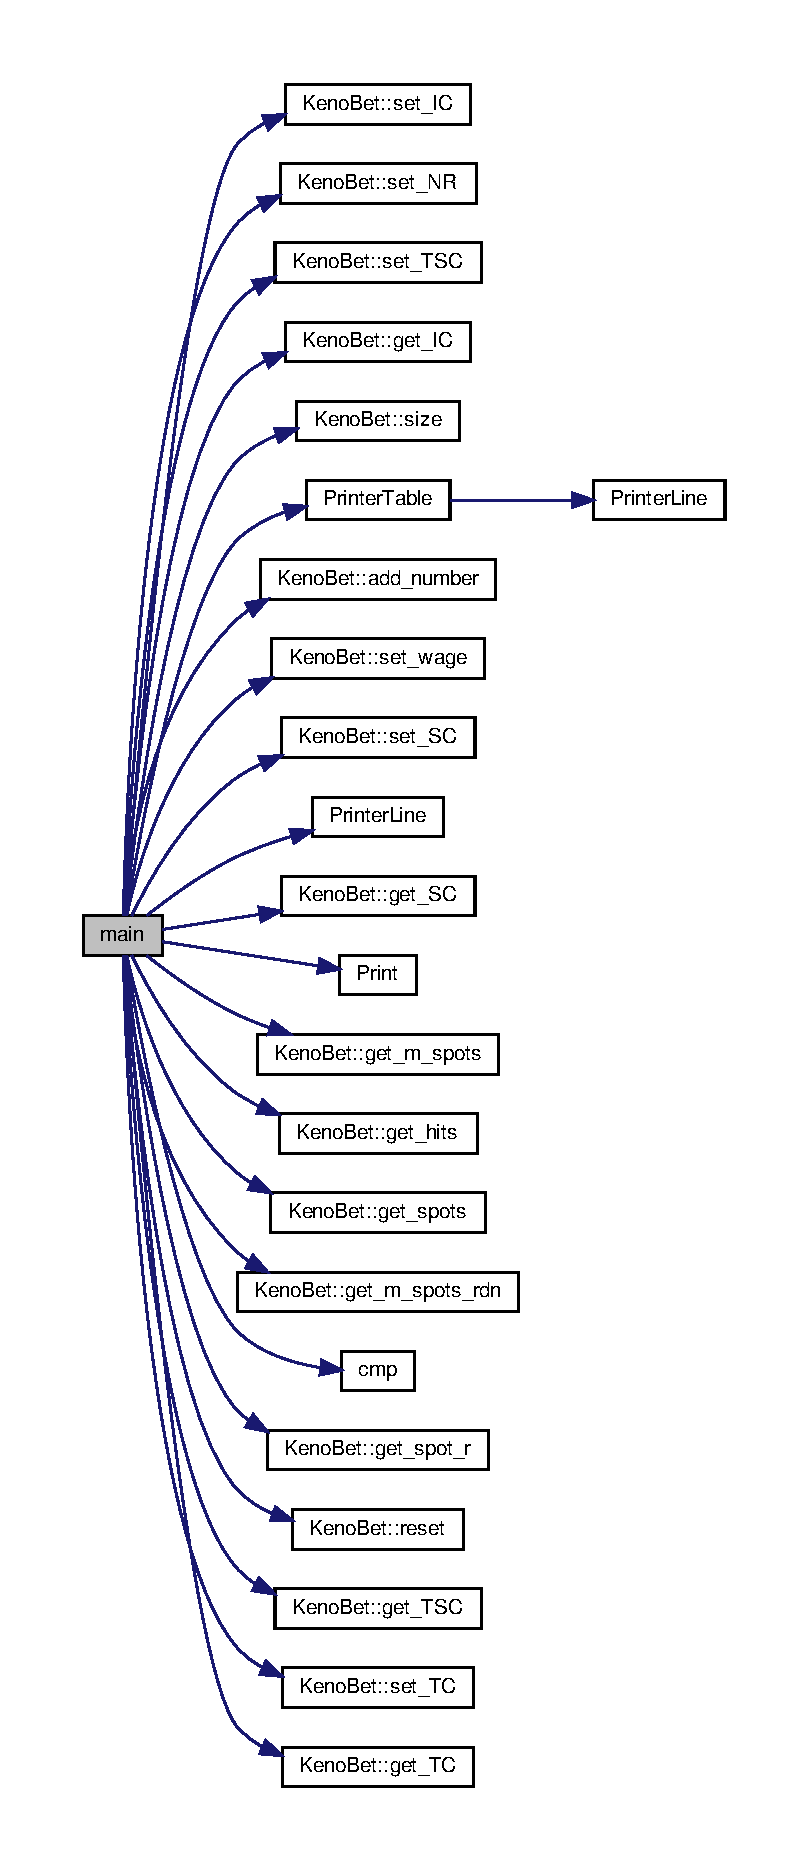
\includegraphics[height=550pt]{main_8cpp_a0ddf1224851353fc92bfbff6f499fa97_cgraph}
\end{center}
\end{figure}

%--- End generated contents ---

% Index
\backmatter
\newpage
\phantomsection
\clearemptydoublepage
\addcontentsline{toc}{chapter}{Index}
\printindex

\end{document}
